\subsubsection{emu}

\begin{figure}[htb!]
    \centering
    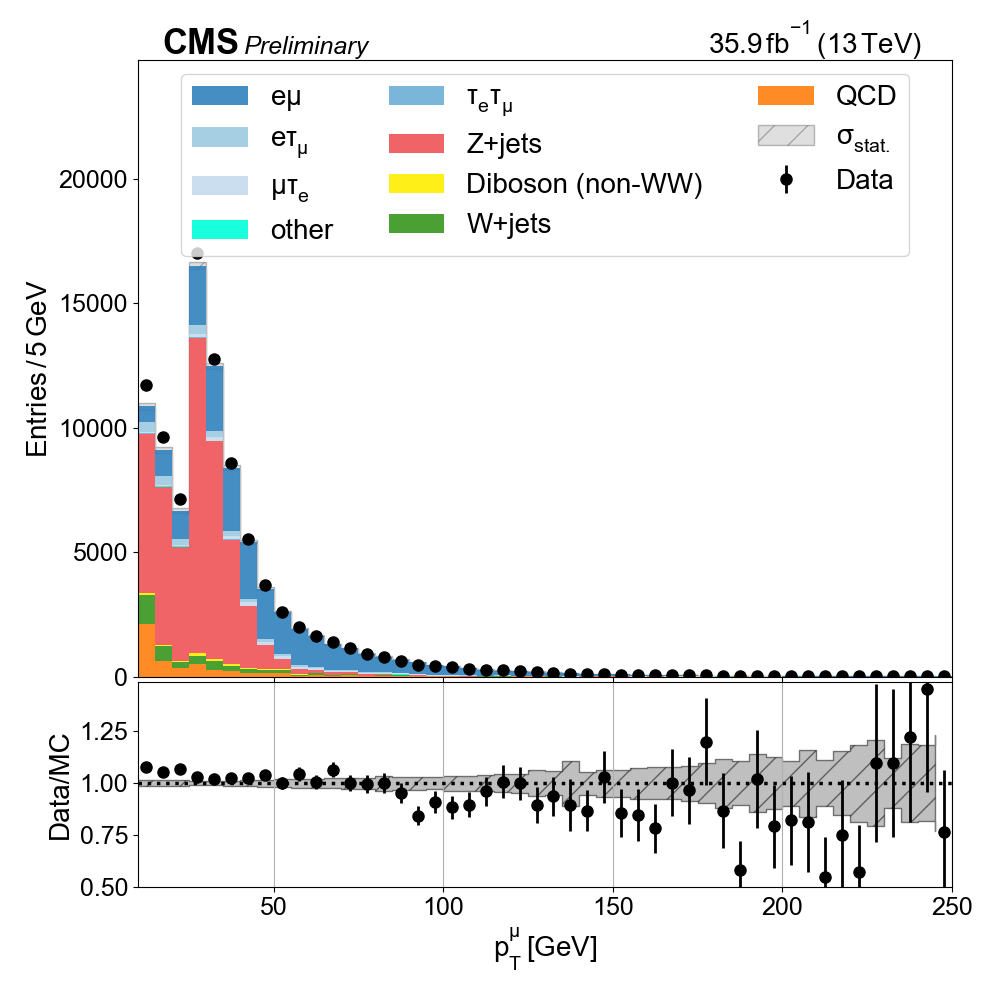
\includegraphics[width=0.4\textwidth]{chapters/Appendix/sectionPlots/figures/data_mc_overlays/emu_2016_cat_eq0_eq0_a_signal_linear_lepton_lepton1_pt}
    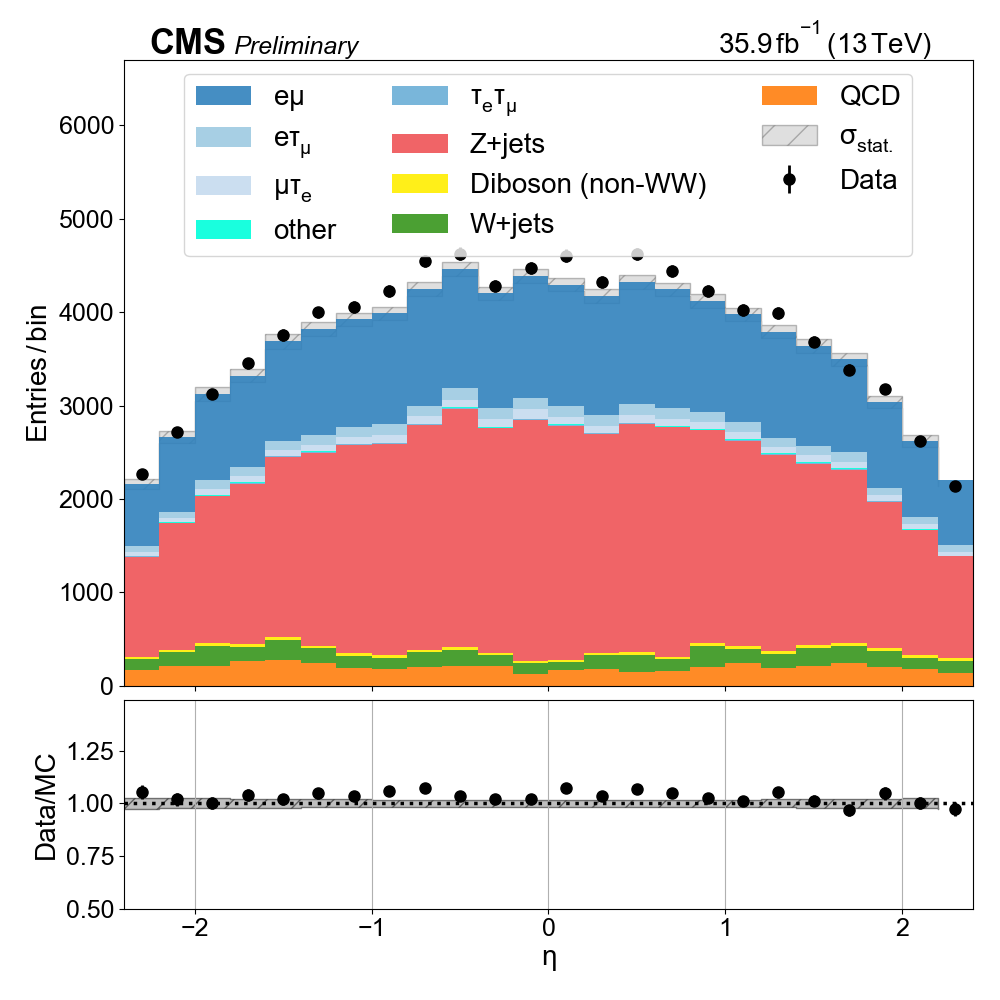
\includegraphics[width=0.4\textwidth]{chapters/Appendix/sectionPlots/figures/data_mc_overlays/emu_2016_cat_eq0_eq0_a_signal_linear_lepton_lepton1_eta}

    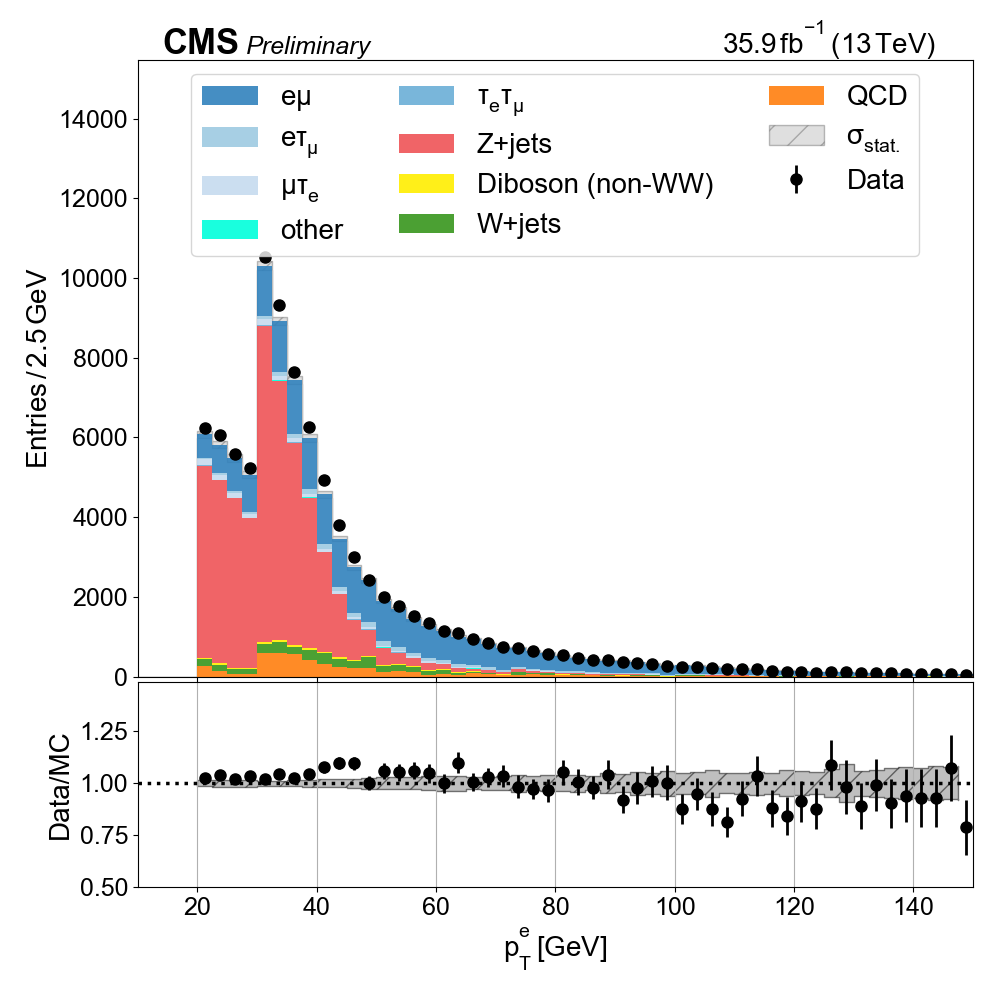
\includegraphics[width=0.4\textwidth]{chapters/Appendix/sectionPlots/figures/data_mc_overlays/emu_2016_cat_eq0_eq0_a_signal_linear_lepton_lepton2_pt}
    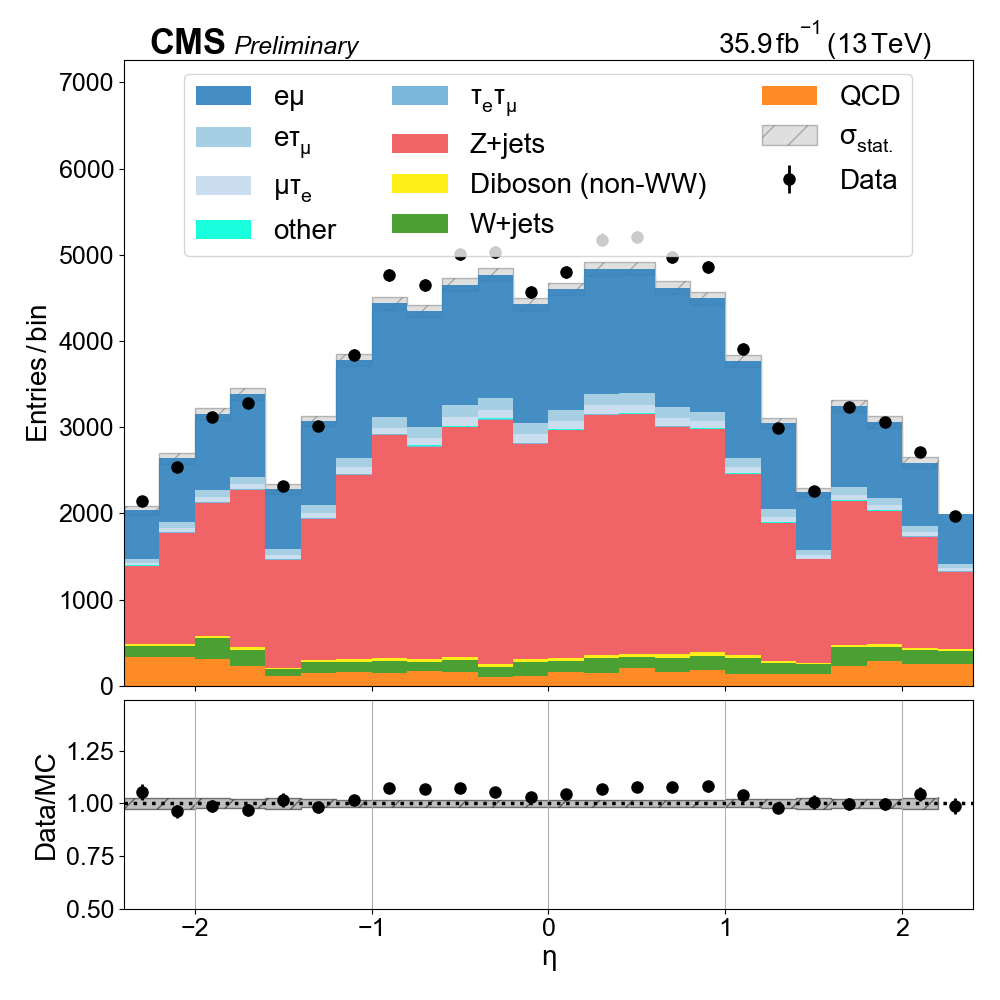
\includegraphics[width=0.4\textwidth]{chapters/Appendix/sectionPlots/figures/data_mc_overlays/emu_2016_cat_eq0_eq0_a_signal_linear_lepton_lepton2_eta}
    \caption{\pt and $\eta$ distributions for leading (top) and trailing
    (bottom) electrons in the $e\mu$ channel with $N_{j} = 0$.}
    \label{fig:emu_1_kinematic}
\end{figure}

\begin{figure}[htb!]
    \centering
    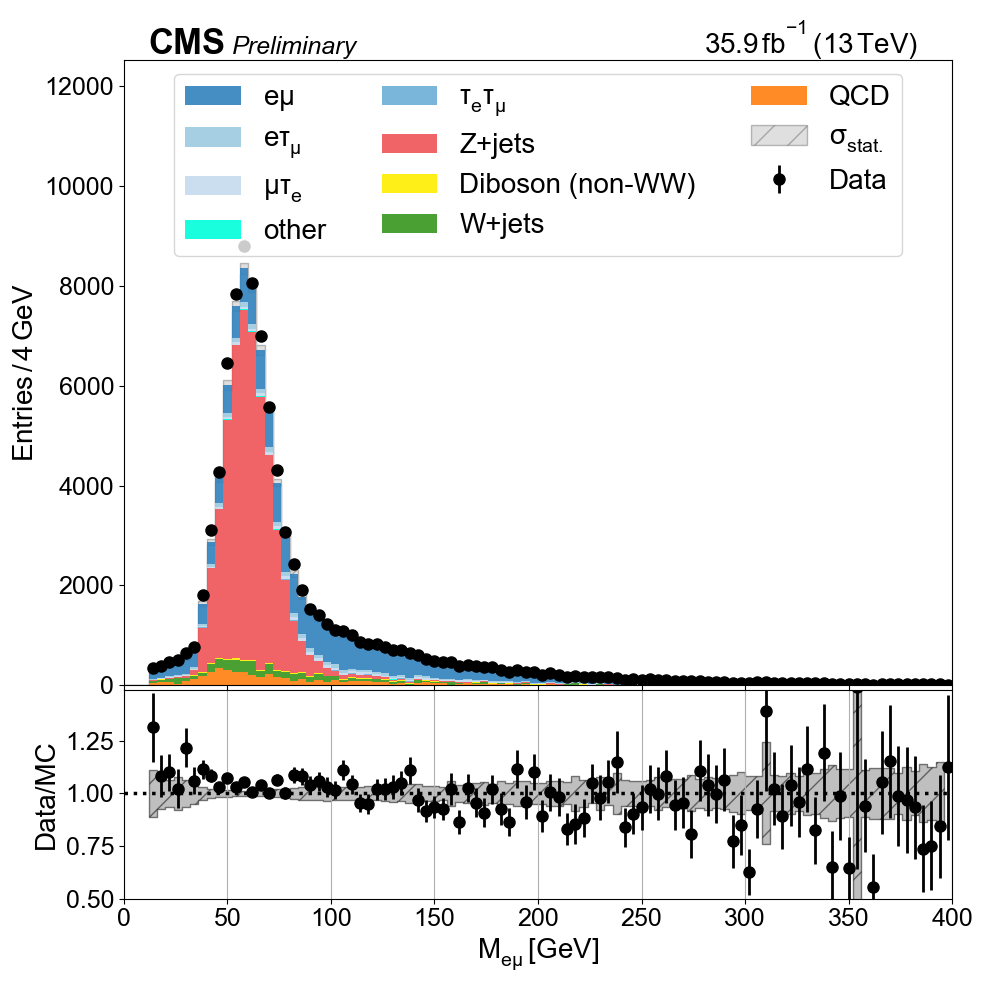
\includegraphics[width=0.3\textwidth]{chapters/Appendix/sectionPlots/figures/data_mc_overlays/emu_2016_cat_eq0_eq0_a_signal_linear_lepton_dilepton1_mass}
    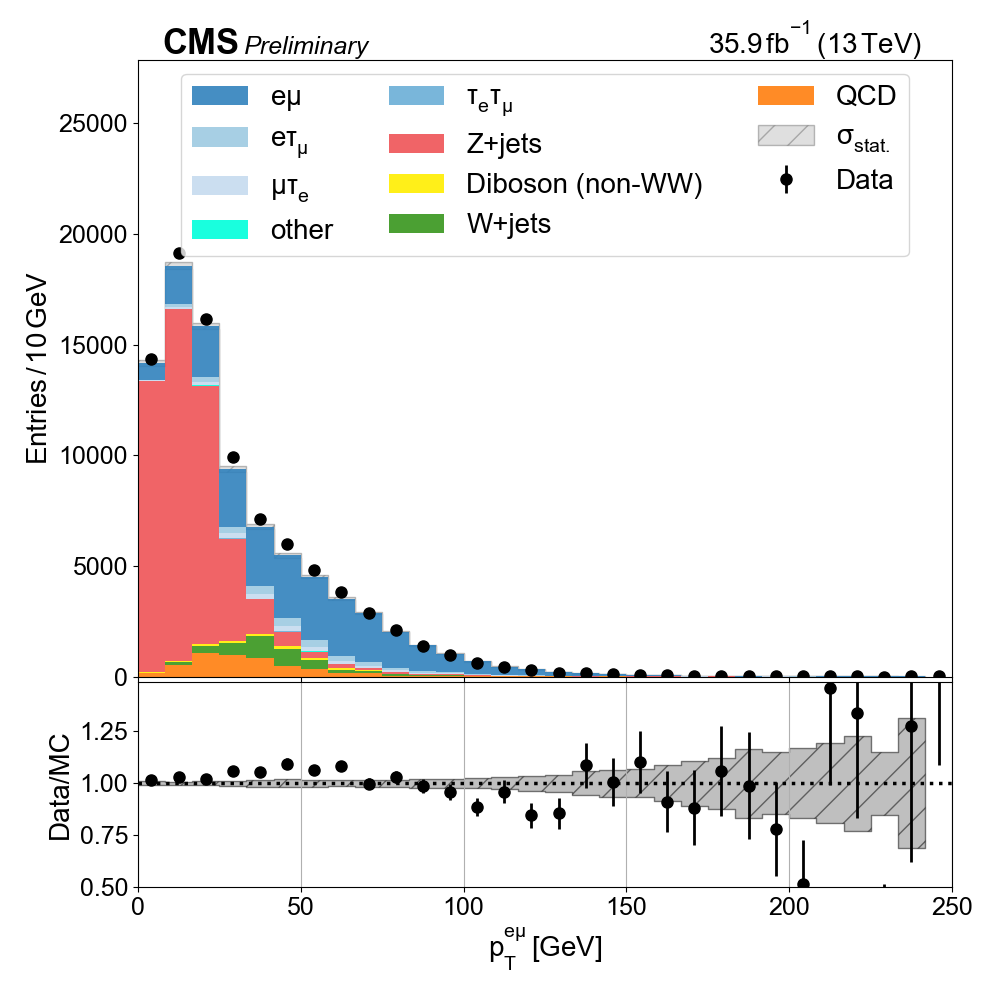
\includegraphics[width=0.3\textwidth]{chapters/Appendix/sectionPlots/figures/data_mc_overlays/emu_2016_cat_eq0_eq0_a_signal_linear_lepton_dilepton1_pt}
    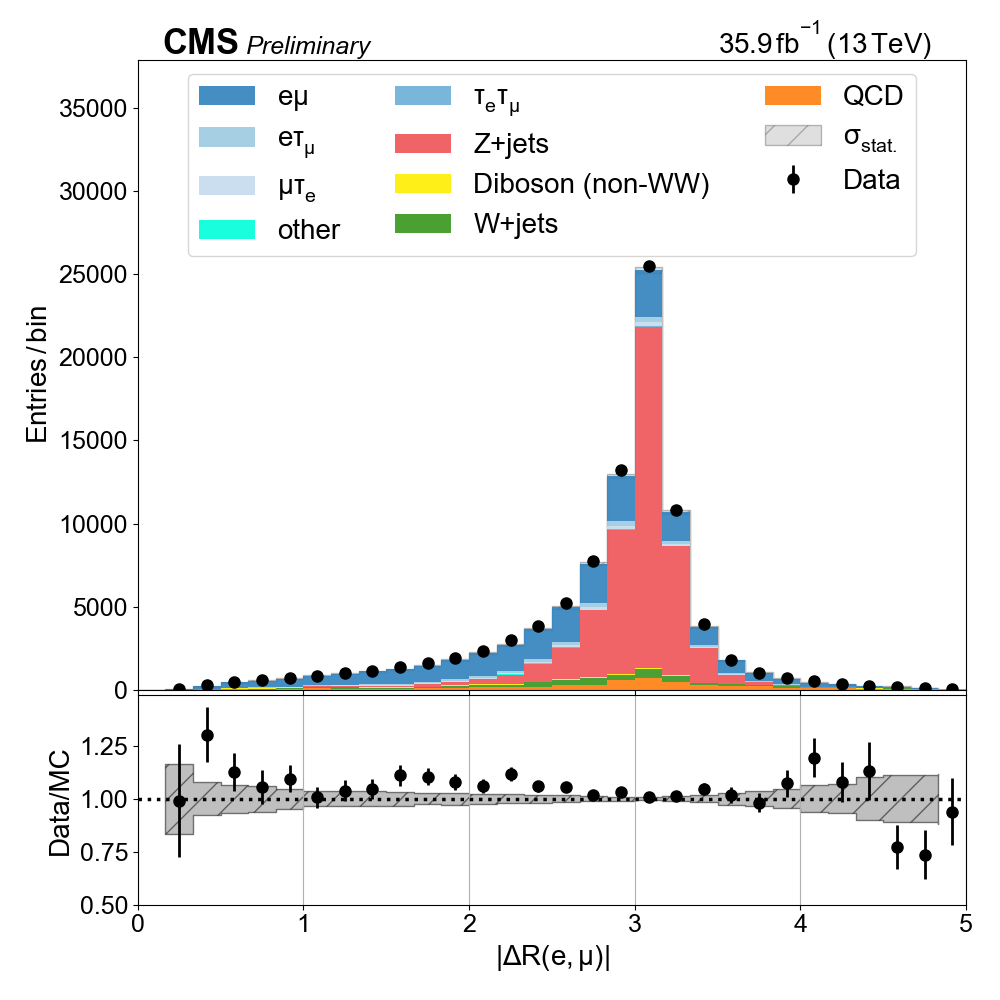
\includegraphics[width=0.3\textwidth]{chapters/Appendix/sectionPlots/figures/data_mc_overlays/emu_2016_cat_eq0_eq0_a_signal_linear_lepton_dilepton1_delta_r}
    \caption{Dielectron mass, \pt, and $\Delta R$ in the $e\mu$ channel
    with $N_{j} = 0$.}
    \label{fig:emu_1_dilepton}
\end{figure}

\begin{figure}[htb!]
    \centering
    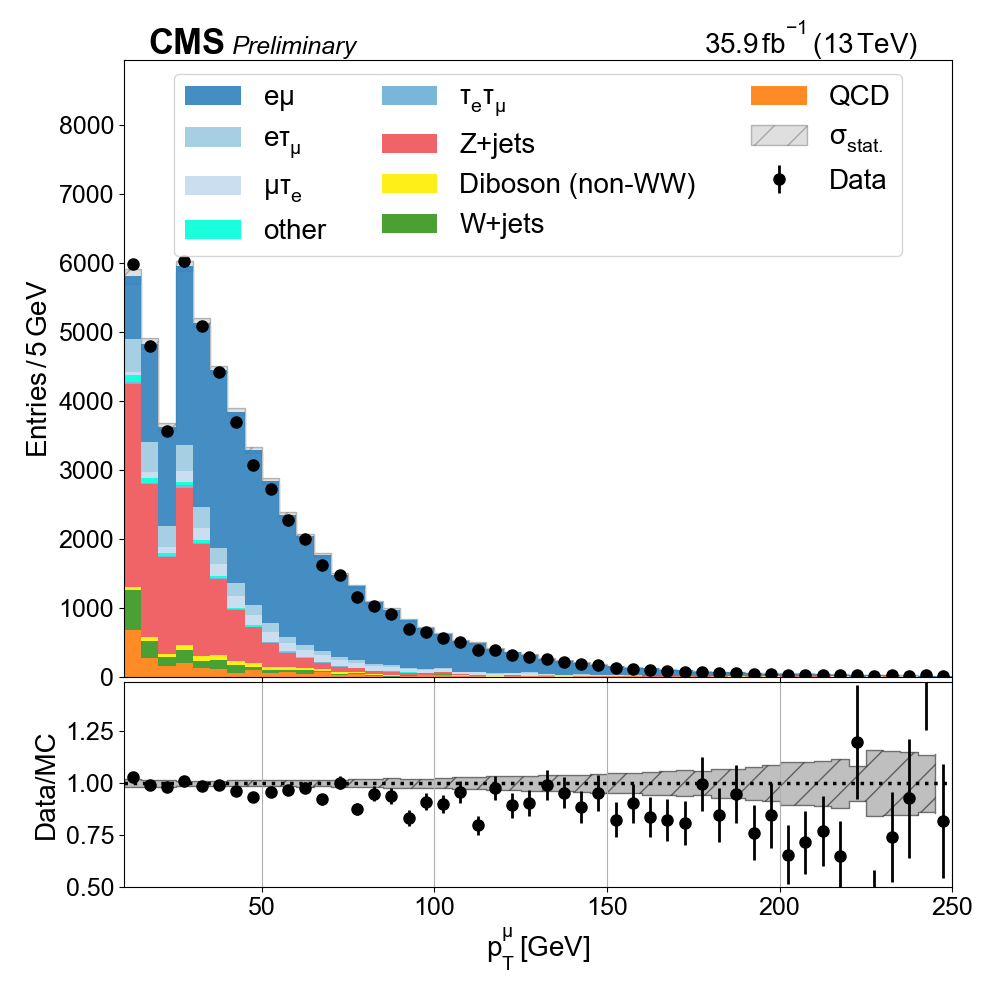
\includegraphics[width=0.4\textwidth]{chapters/Appendix/sectionPlots/figures/data_mc_overlays/emu_2016_cat_eq1_eq0_a_signal_linear_lepton_lepton1_pt}
    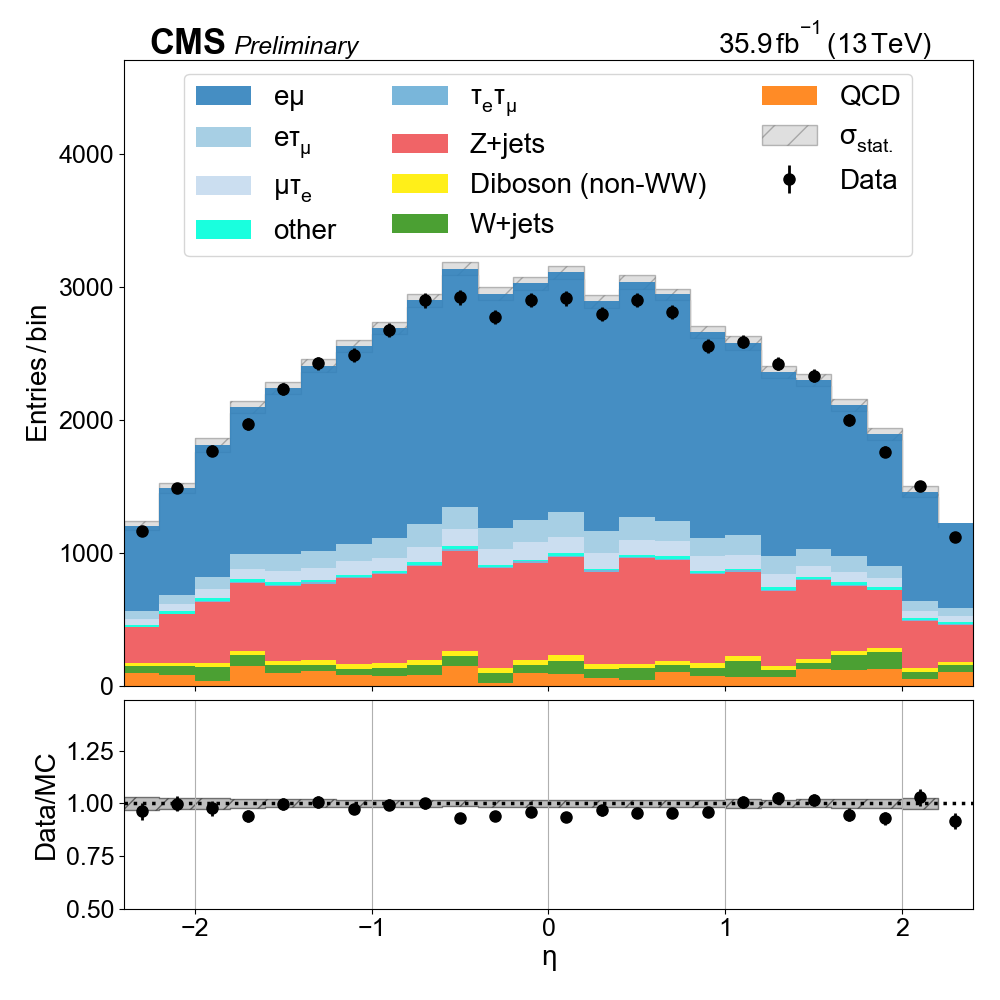
\includegraphics[width=0.4\textwidth]{chapters/Appendix/sectionPlots/figures/data_mc_overlays/emu_2016_cat_eq1_eq0_a_signal_linear_lepton_lepton1_eta}

    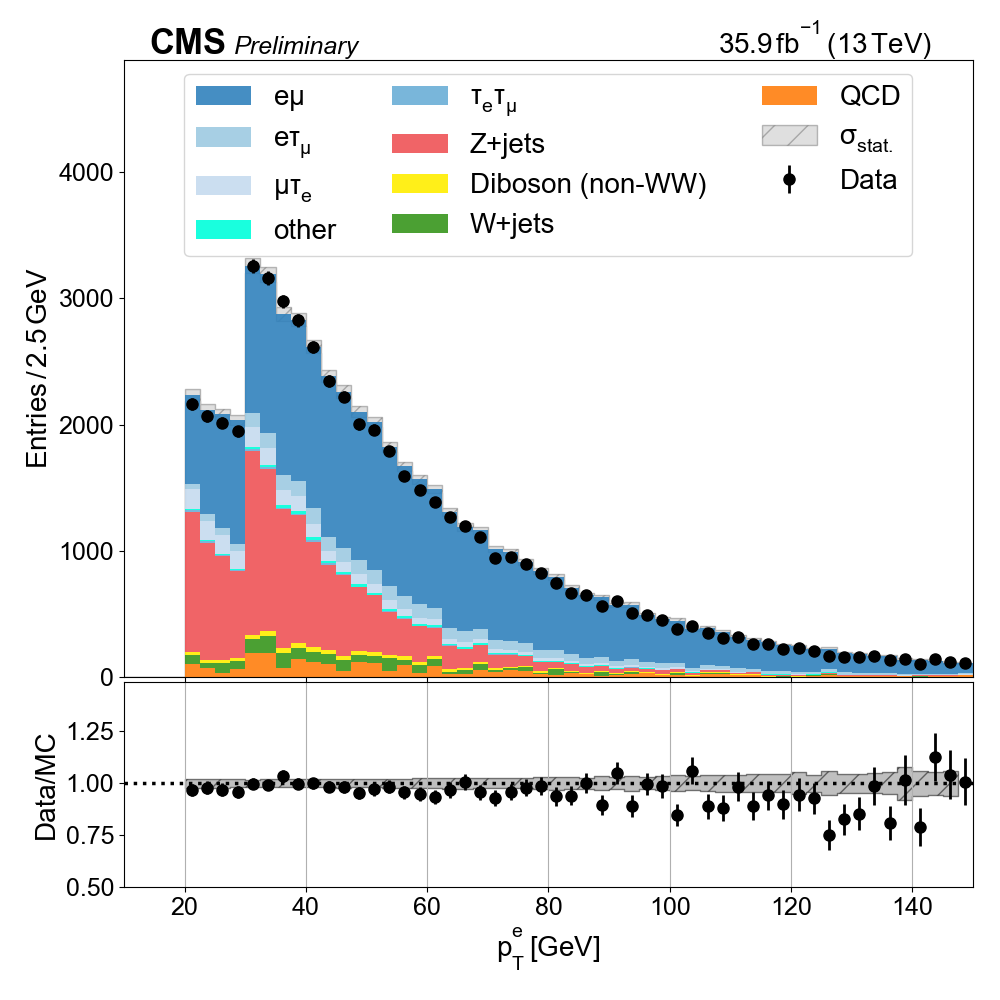
\includegraphics[width=0.4\textwidth]{chapters/Appendix/sectionPlots/figures/data_mc_overlays/emu_2016_cat_eq1_eq0_a_signal_linear_lepton_lepton2_pt}
    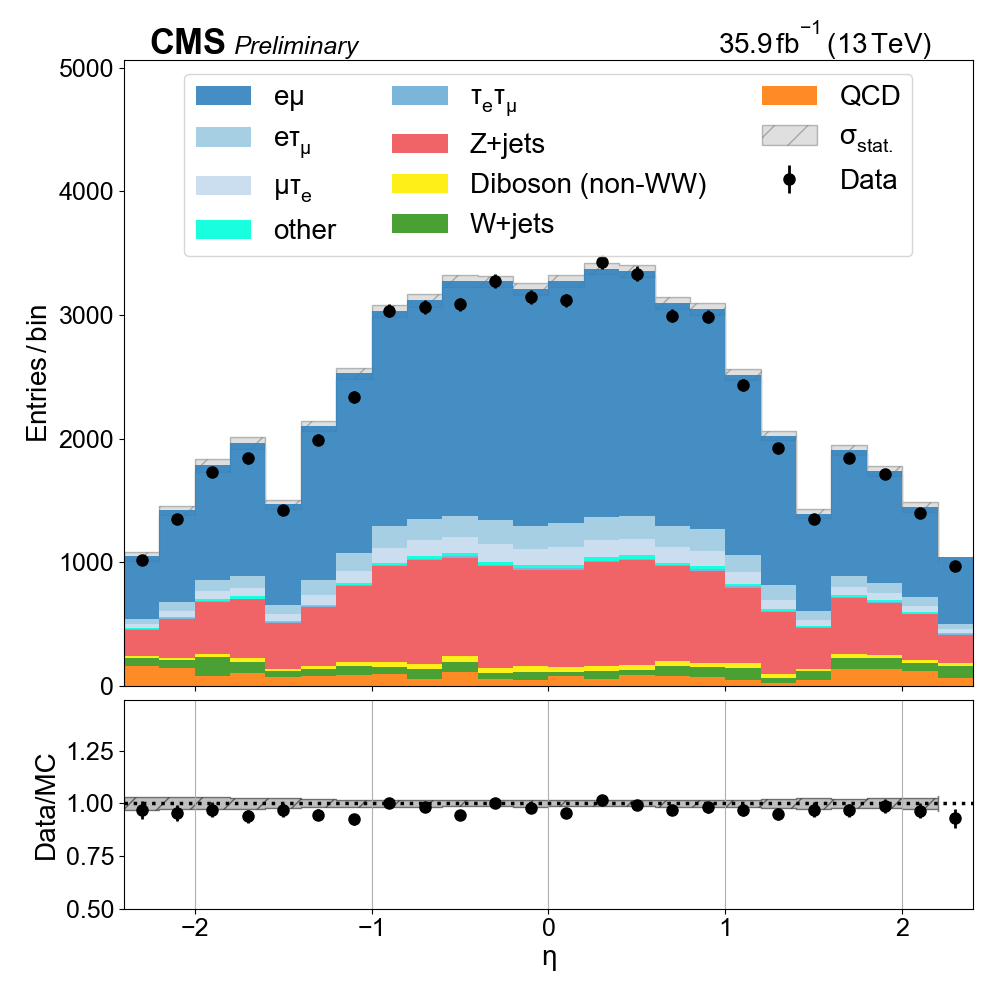
\includegraphics[width=0.4\textwidth]{chapters/Appendix/sectionPlots/figures/data_mc_overlays/emu_2016_cat_eq1_eq0_a_signal_linear_lepton_lepton2_eta}
    \caption{\pt and $\eta$ distributions for leading (top) and trailing
        (bottom) electrons in the $e\mu$ channel with $N_{j} = 1$ and
        $N_{b} = 0$.}
    \label{fig:emu_2_kinematic}
\end{figure}

\begin{figure}[htb!]
    \centering
    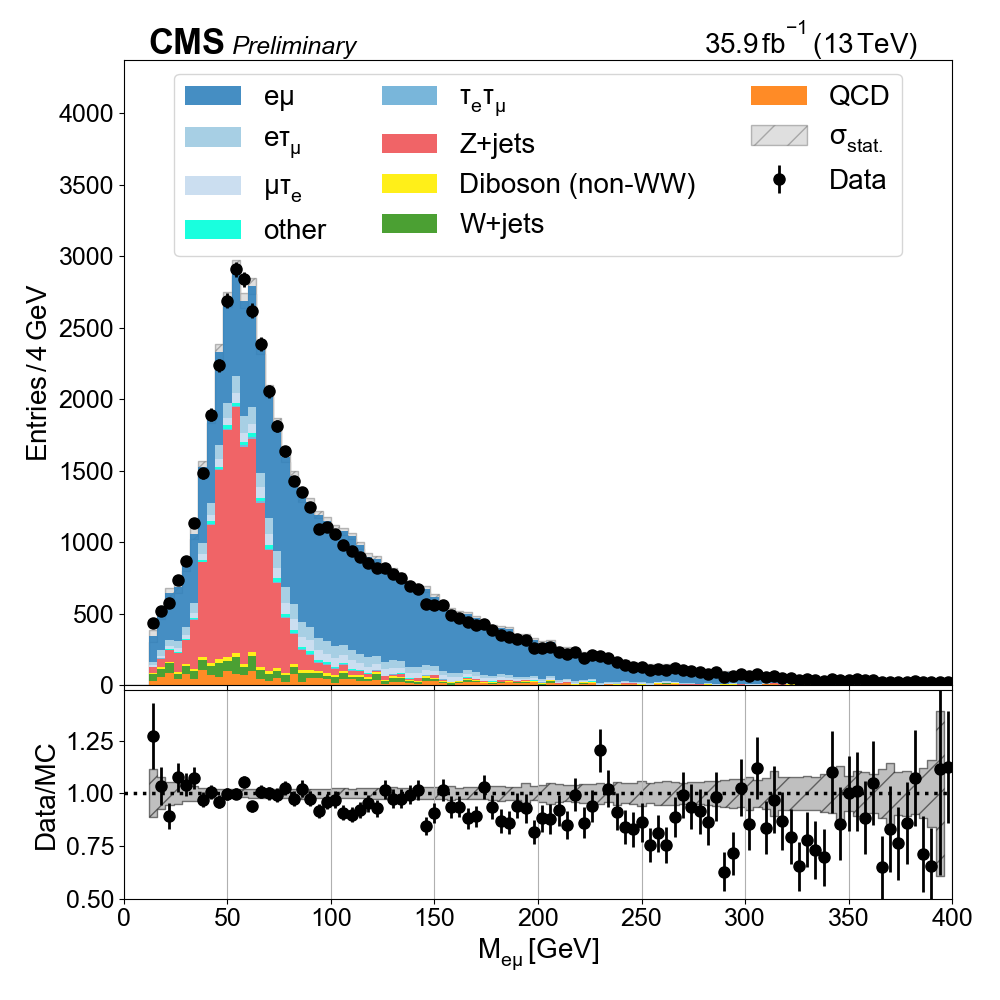
\includegraphics[width=0.3\textwidth]{chapters/Appendix/sectionPlots/figures/data_mc_overlays/emu_2016_cat_eq1_eq0_a_signal_linear_lepton_dilepton1_mass}
    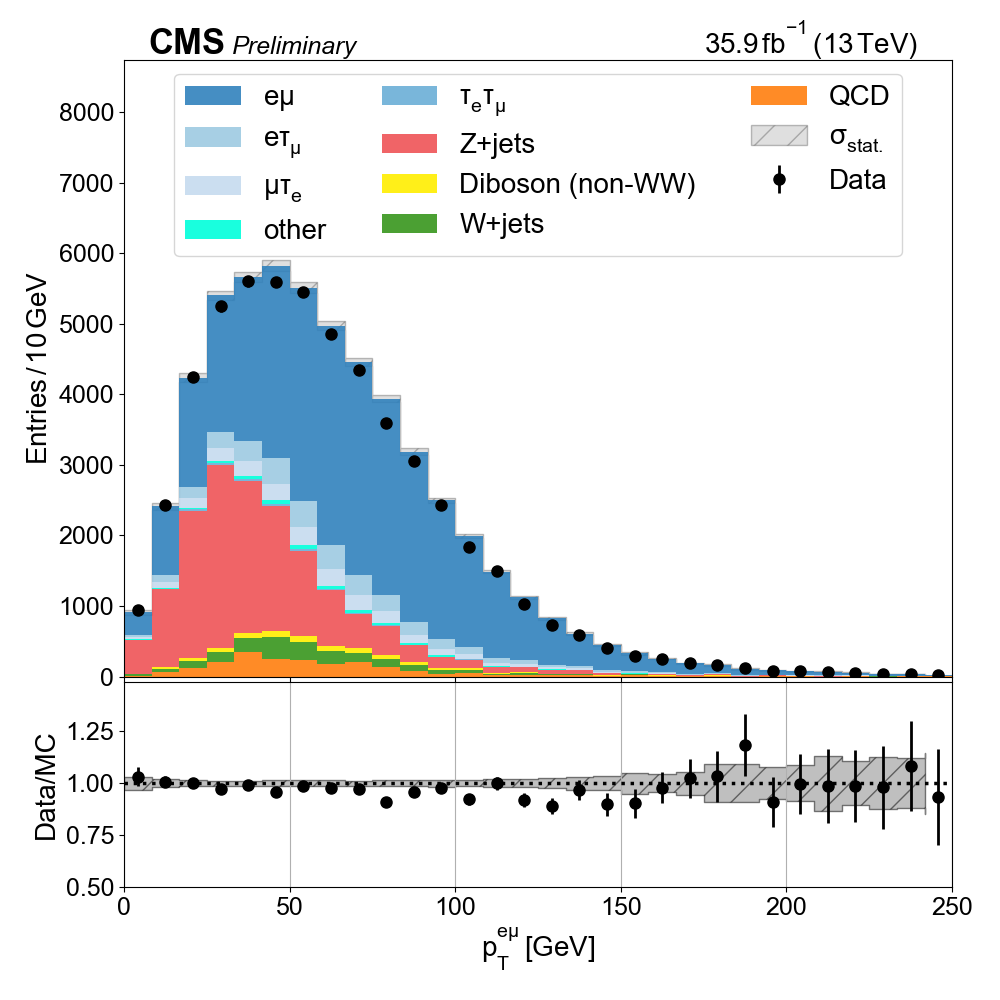
\includegraphics[width=0.3\textwidth]{chapters/Appendix/sectionPlots/figures/data_mc_overlays/emu_2016_cat_eq1_eq0_a_signal_linear_lepton_dilepton1_pt}
    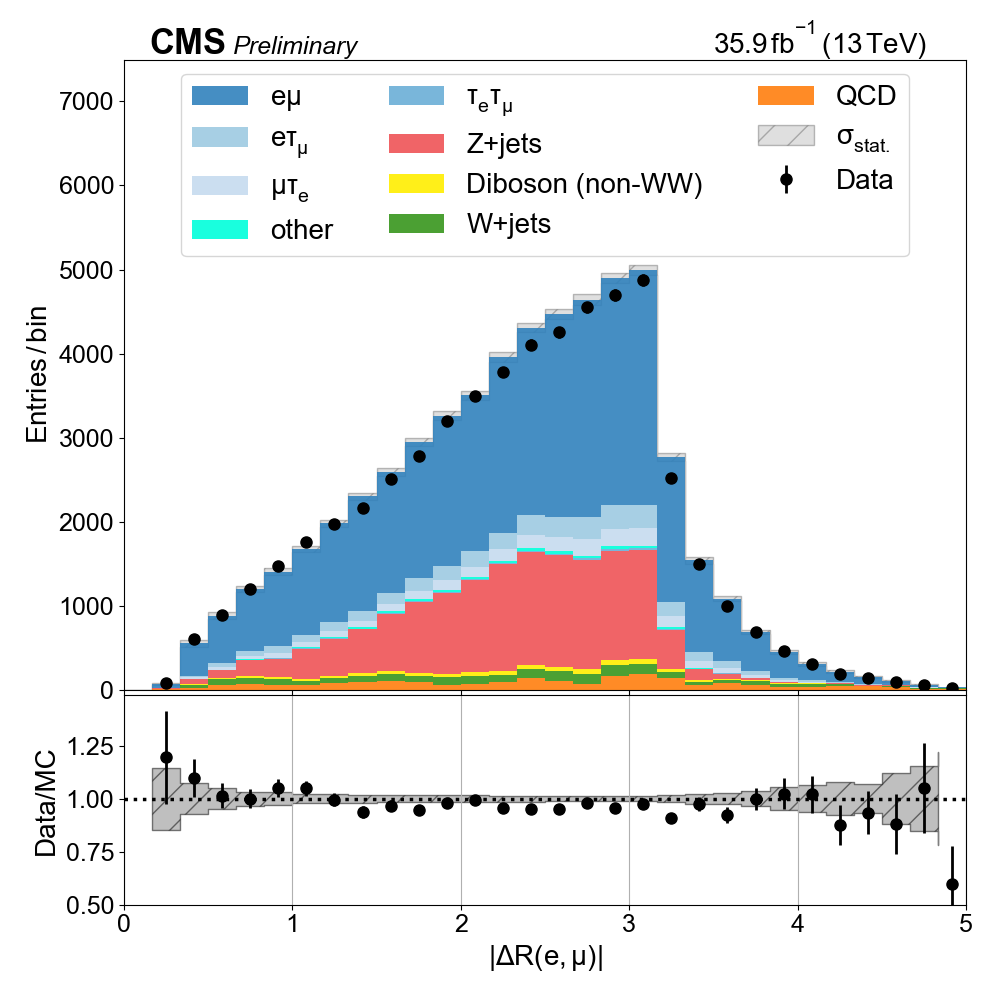
\includegraphics[width=0.3\textwidth]{chapters/Appendix/sectionPlots/figures/data_mc_overlays/emu_2016_cat_eq1_eq0_a_signal_linear_lepton_dilepton1_delta_r}
    \caption{Dielectron mass, \pt, and $\Delta R$ in the $e\mu$ channel
    with $N_{j} = 0$ and $N_{b} = 0$.}
    \label{fig:emu_2_dilepton}
\end{figure}

\begin{figure}[htb!]
    \centering
    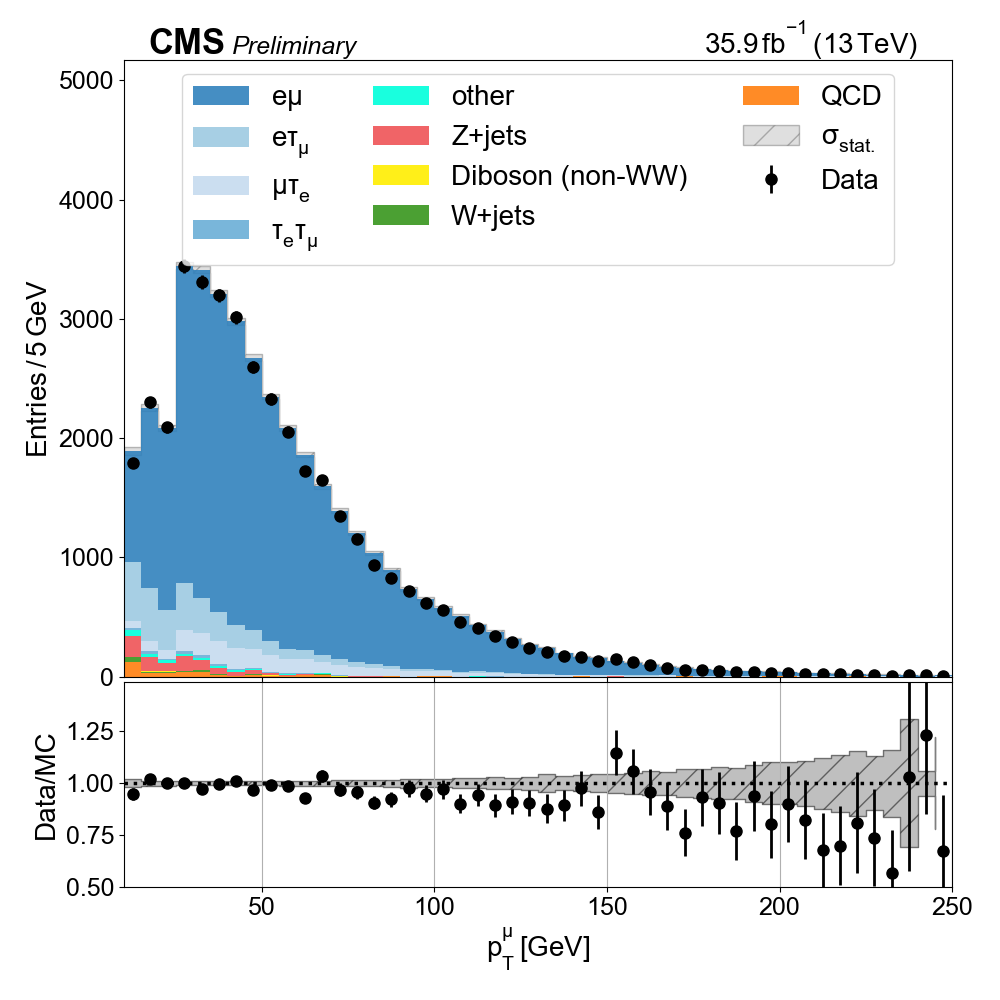
\includegraphics[width=0.4\textwidth]{chapters/Appendix/sectionPlots/figures/data_mc_overlays/emu_2016_cat_eq1_eq1_a_signal_linear_lepton_lepton1_pt}
    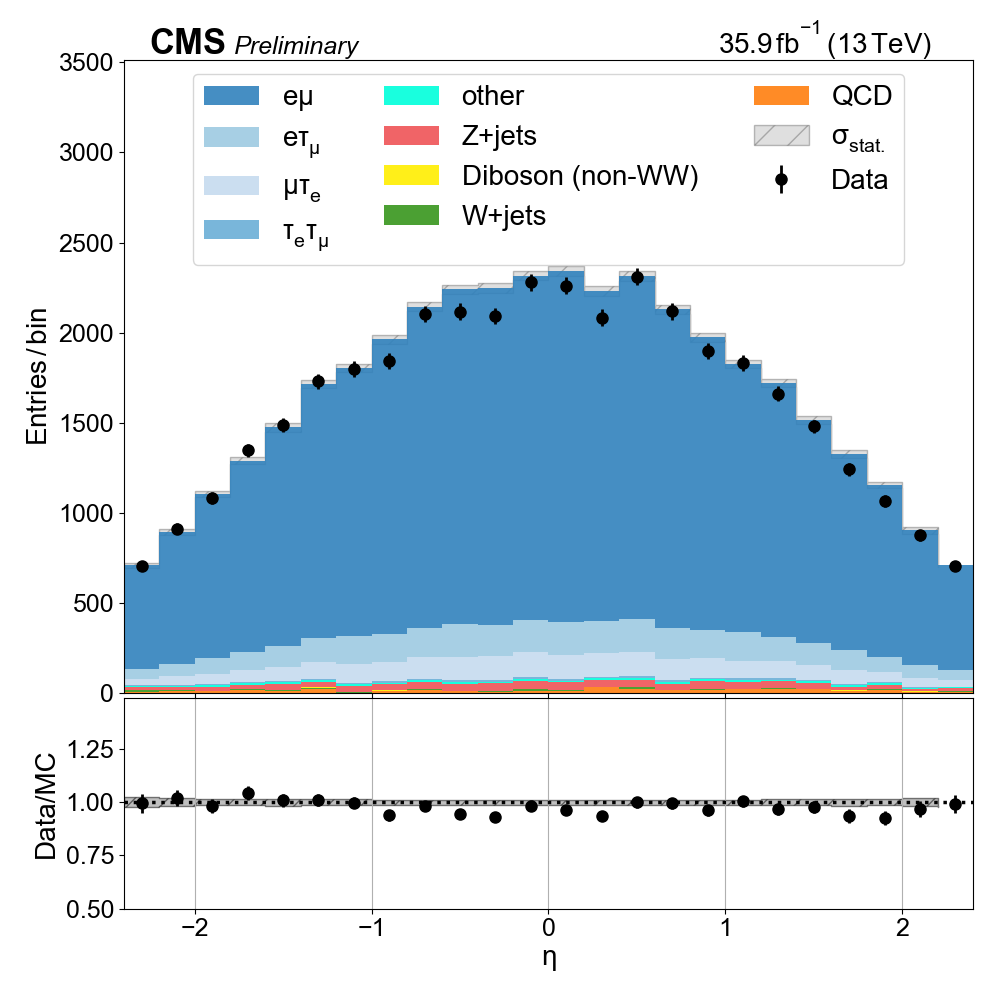
\includegraphics[width=0.4\textwidth]{chapters/Appendix/sectionPlots/figures/data_mc_overlays/emu_2016_cat_eq1_eq1_a_signal_linear_lepton_lepton1_eta}

    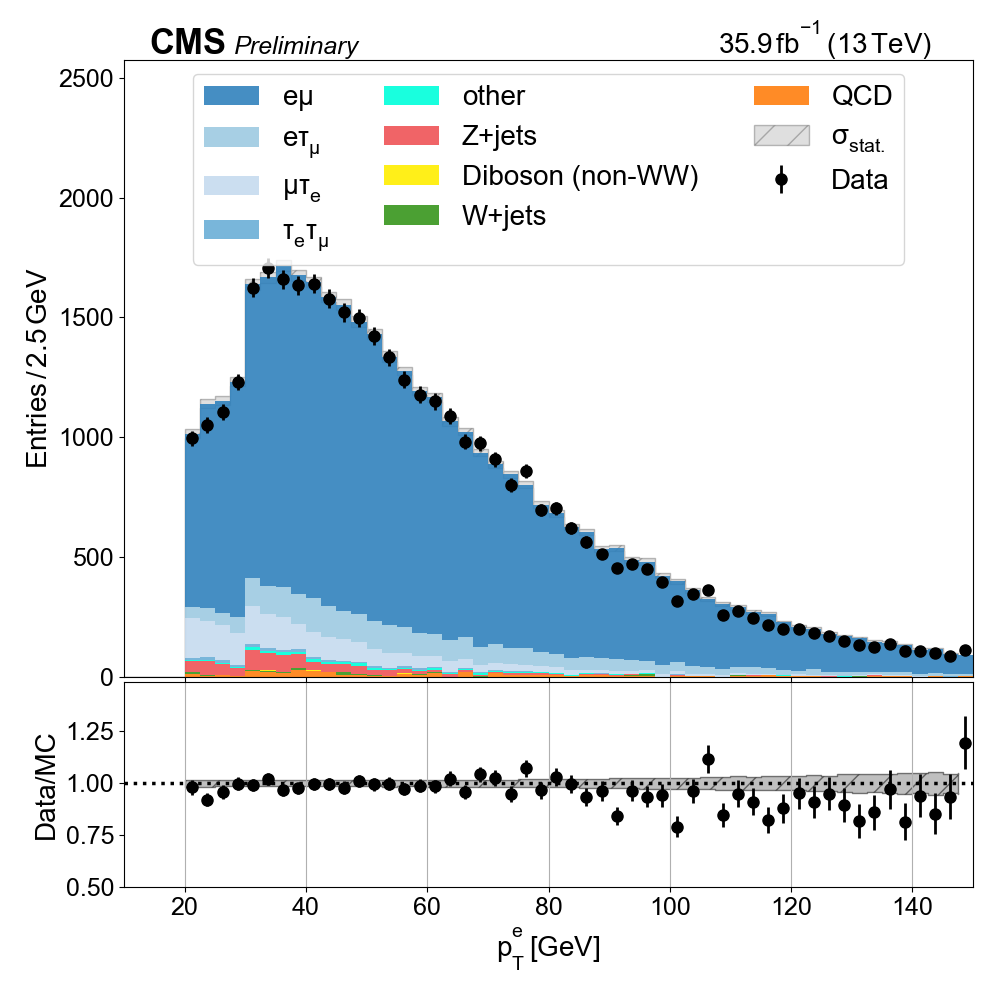
\includegraphics[width=0.4\textwidth]{chapters/Appendix/sectionPlots/figures/data_mc_overlays/emu_2016_cat_eq1_eq1_a_signal_linear_lepton_lepton2_pt}
    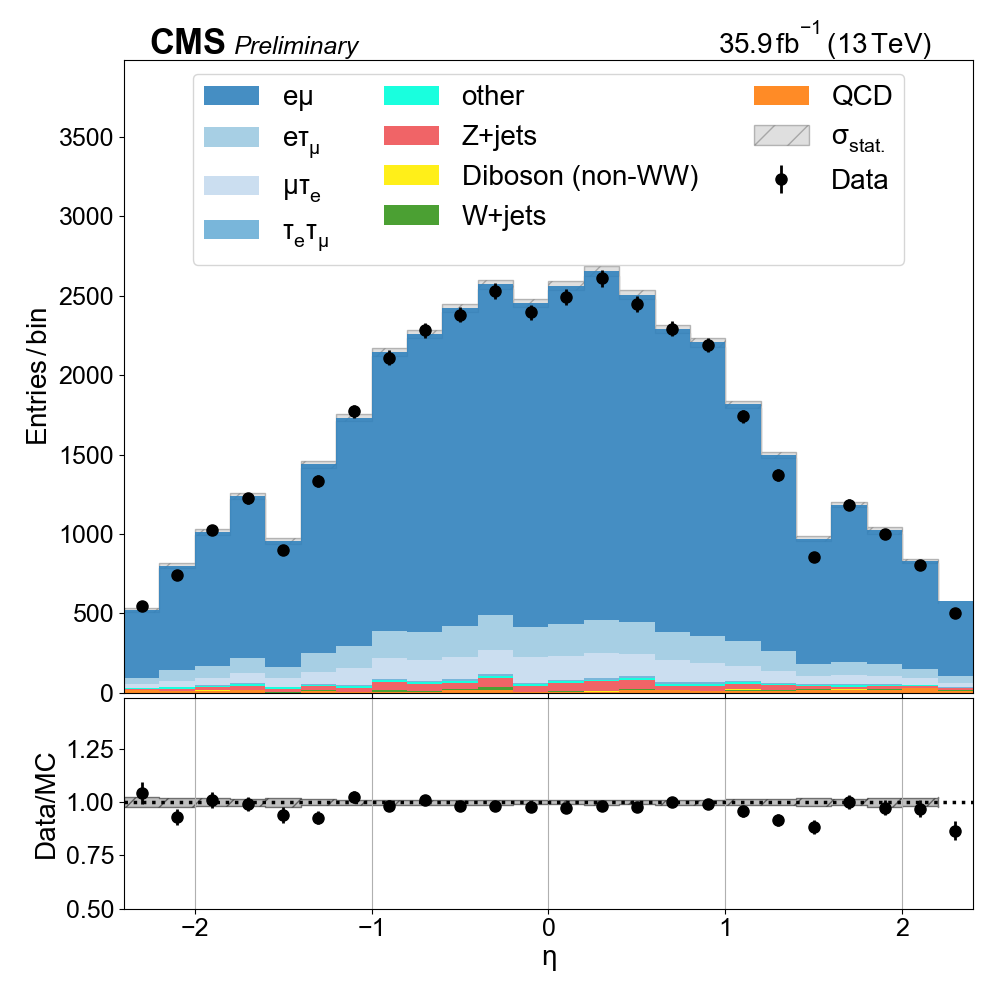
\includegraphics[width=0.4\textwidth]{chapters/Appendix/sectionPlots/figures/data_mc_overlays/emu_2016_cat_eq1_eq1_a_signal_linear_lepton_lepton2_eta}
    \caption{\pt and $\eta$ distributions for leading (top) and trailing
        (bottom) electrons in the $e\mu$ channel with $N_{j} = 1$ and
        $N_{b} = 1$.}
    \label{fig:emu_3_kinematic}
\end{figure}

\begin{figure}[htb!]
    \centering
    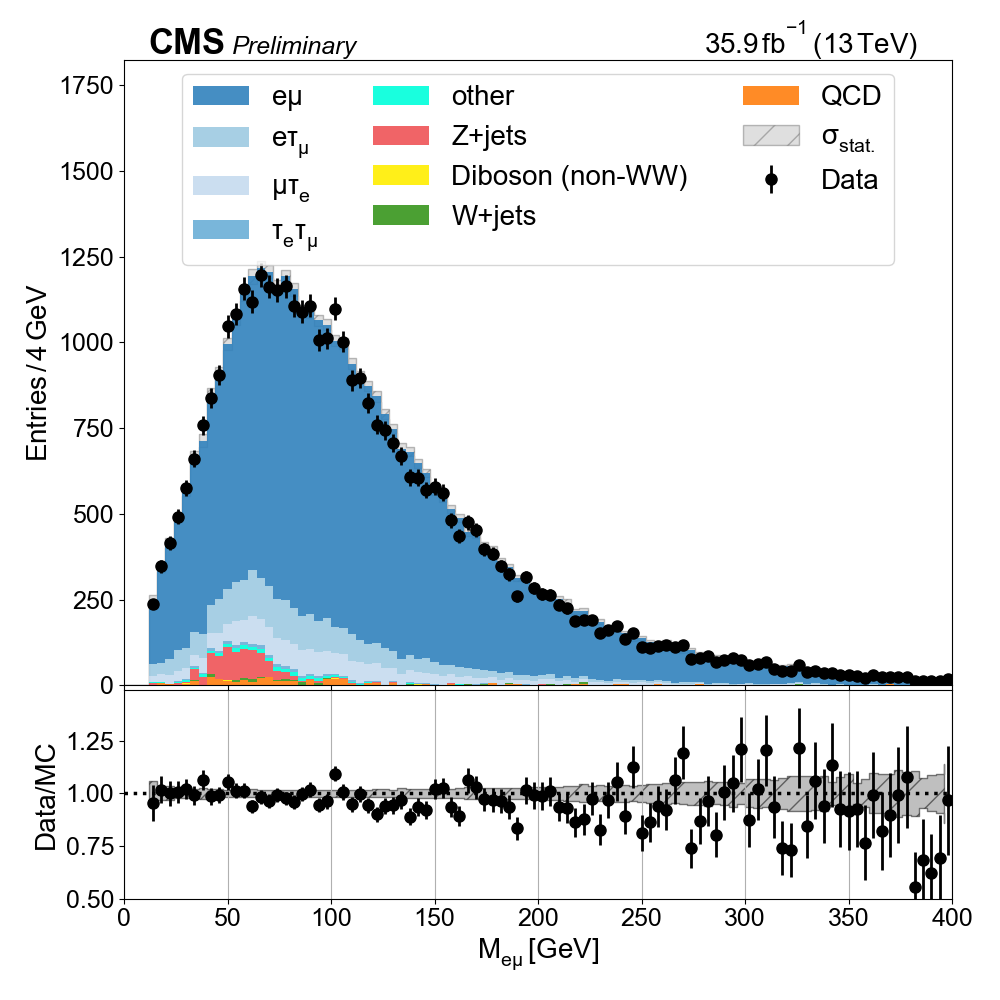
\includegraphics[width=0.3\textwidth]{chapters/Appendix/sectionPlots/figures/data_mc_overlays/emu_2016_cat_eq1_eq1_a_signal_linear_lepton_dilepton1_mass}
    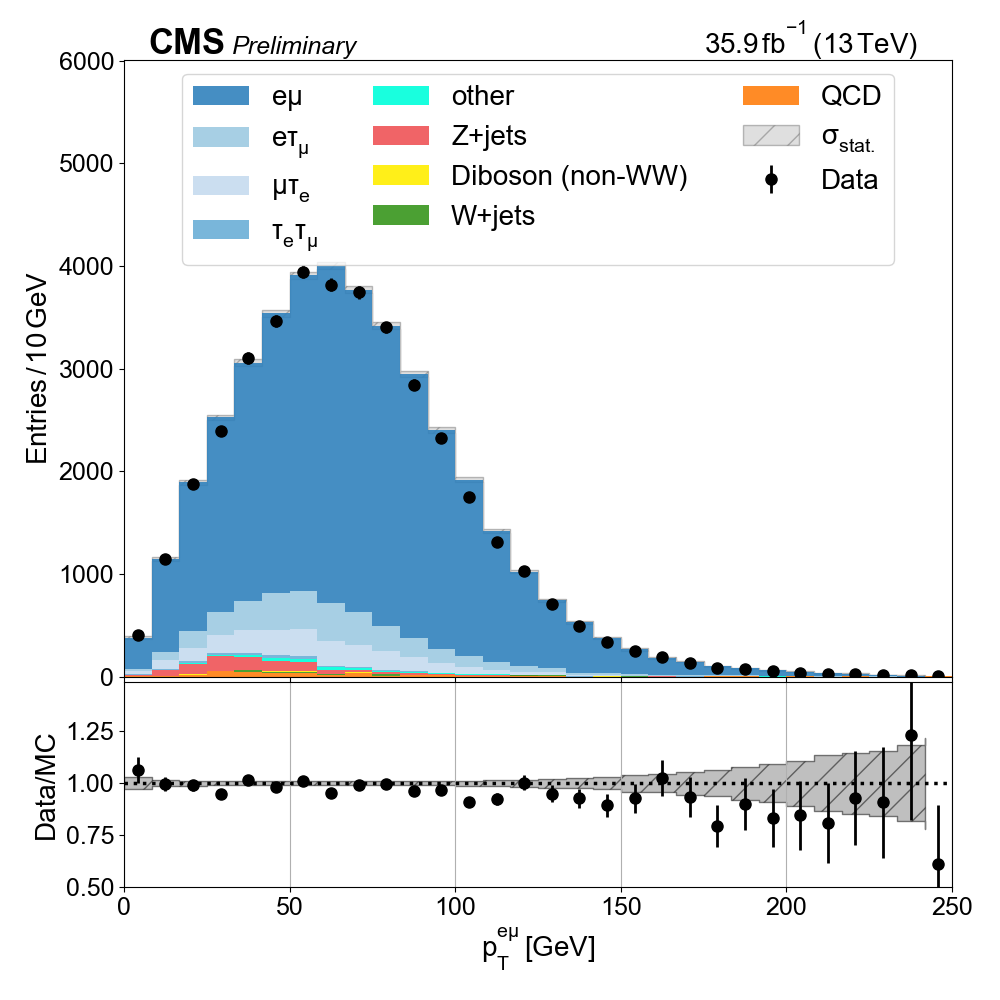
\includegraphics[width=0.3\textwidth]{chapters/Appendix/sectionPlots/figures/data_mc_overlays/emu_2016_cat_eq1_eq1_a_signal_linear_lepton_dilepton1_pt}
    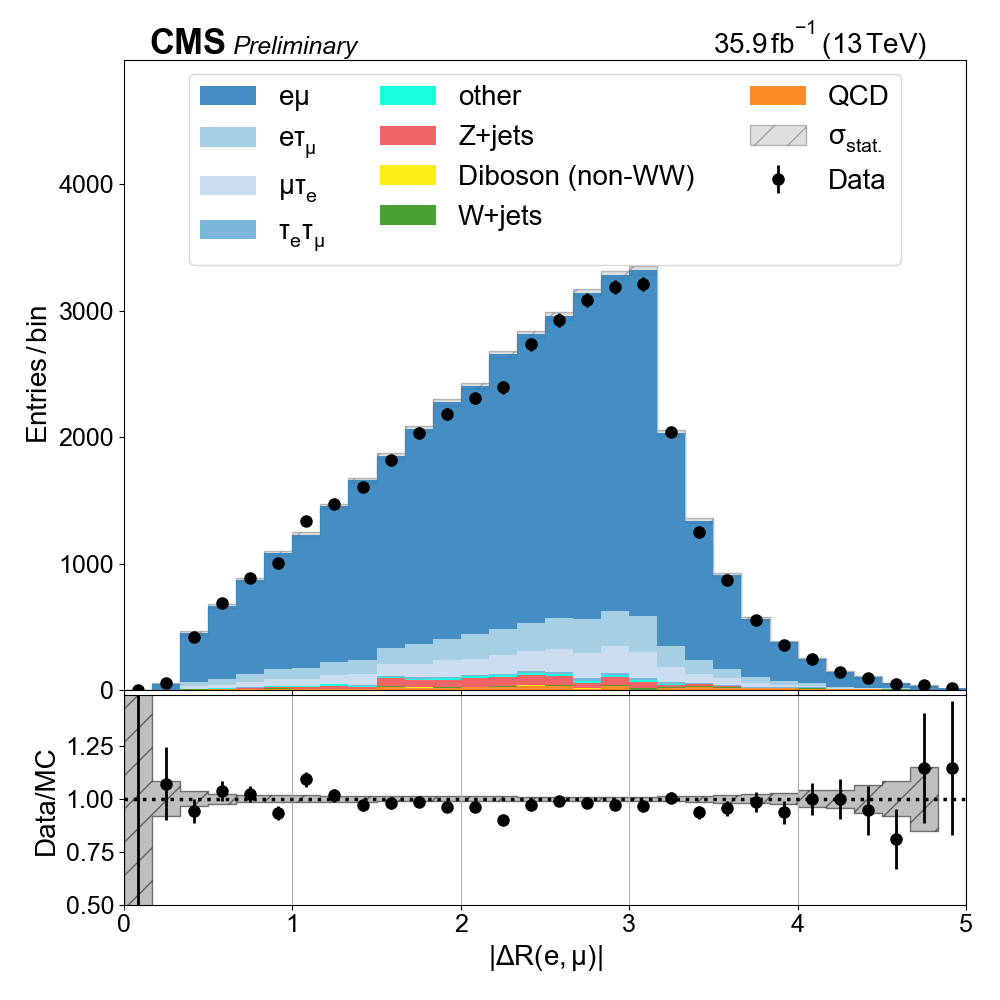
\includegraphics[width=0.3\textwidth]{chapters/Appendix/sectionPlots/figures/data_mc_overlays/emu_2016_cat_eq1_eq1_a_signal_linear_lepton_dilepton1_delta_r}
    \caption{Dielectron mass, \pt, and $\Delta R$ in the $e\mu$ channel
    with $N_{j} = 1$ and $N_{b} = 1$.}
    \label{fig:emu_3_dilepton}
\end{figure}

\begin{figure}[htb!]
    \centering
    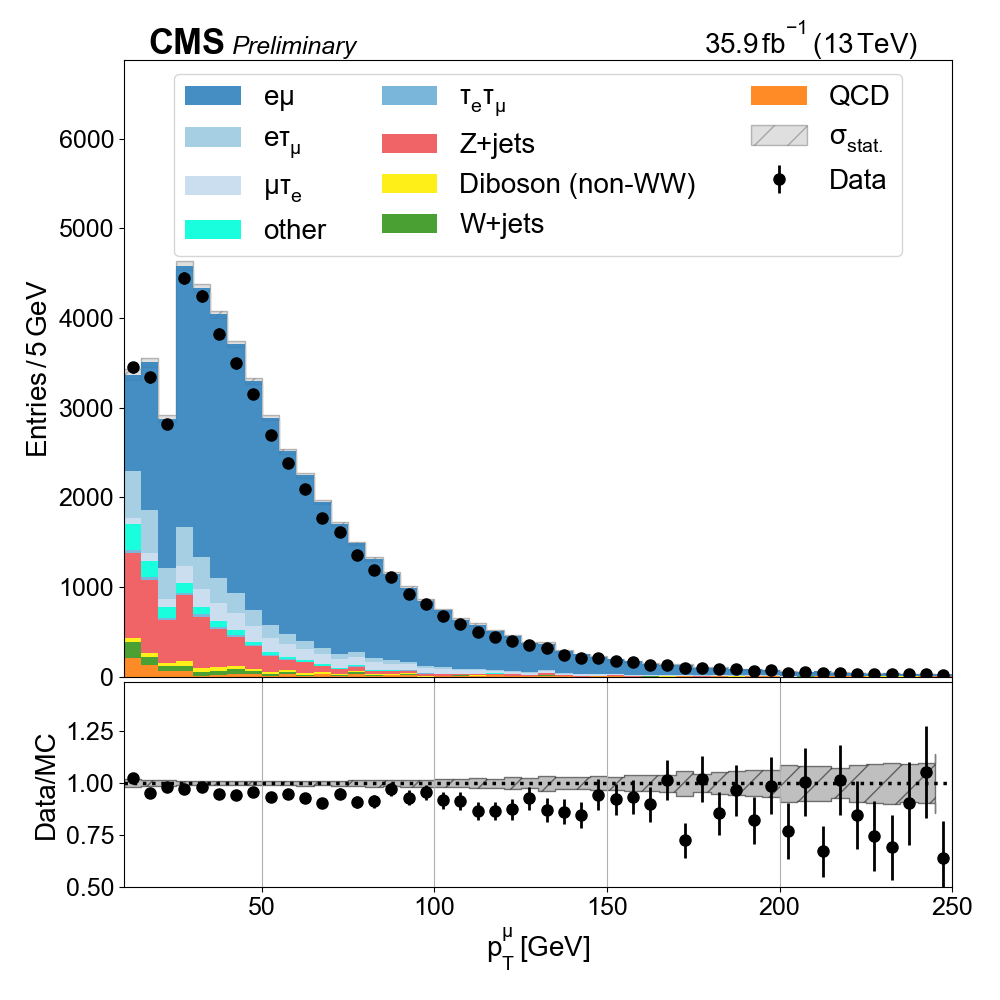
\includegraphics[width=0.4\textwidth]{chapters/Appendix/sectionPlots/figures/data_mc_overlays/emu_2016_cat_gt2_eq0_signal_linear_lepton_lepton1_pt}
    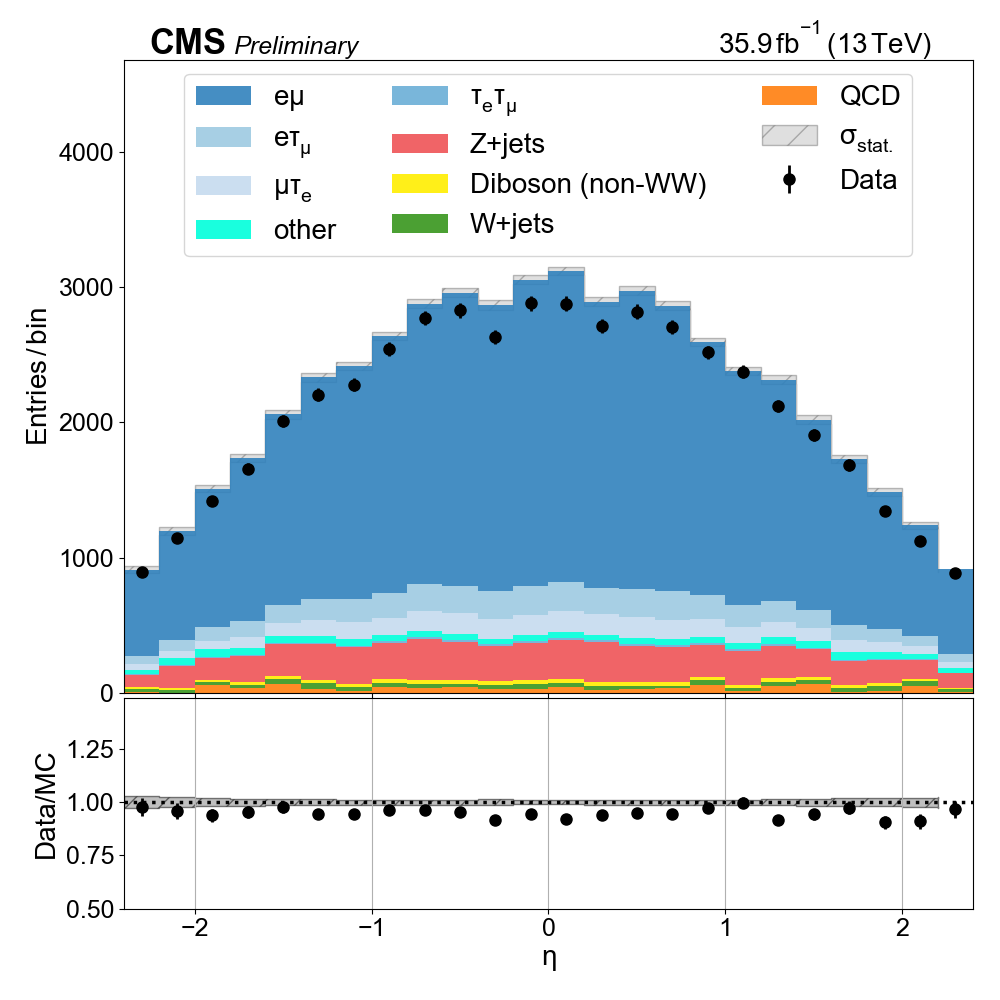
\includegraphics[width=0.4\textwidth]{chapters/Appendix/sectionPlots/figures/data_mc_overlays/emu_2016_cat_gt2_eq0_signal_linear_lepton_lepton1_eta}

    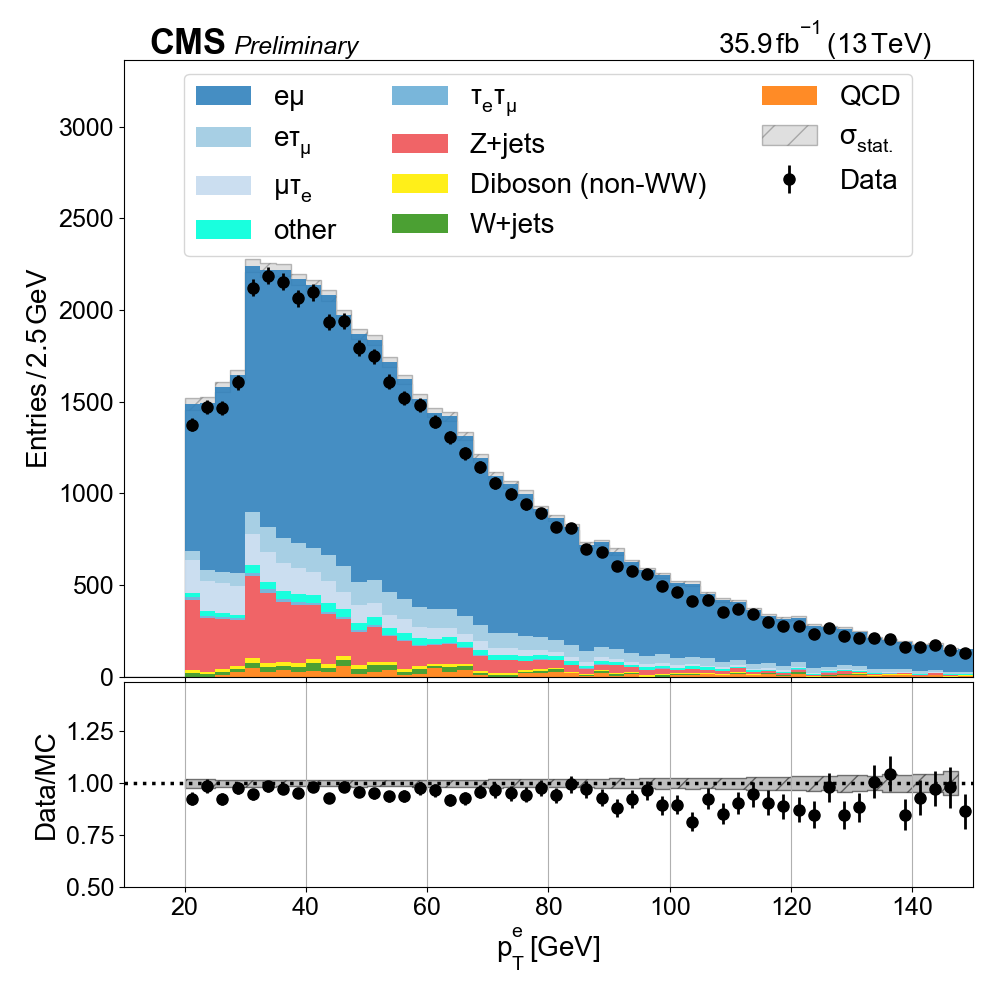
\includegraphics[width=0.4\textwidth]{chapters/Appendix/sectionPlots/figures/data_mc_overlays/emu_2016_cat_gt2_eq0_signal_linear_lepton_lepton2_pt}
    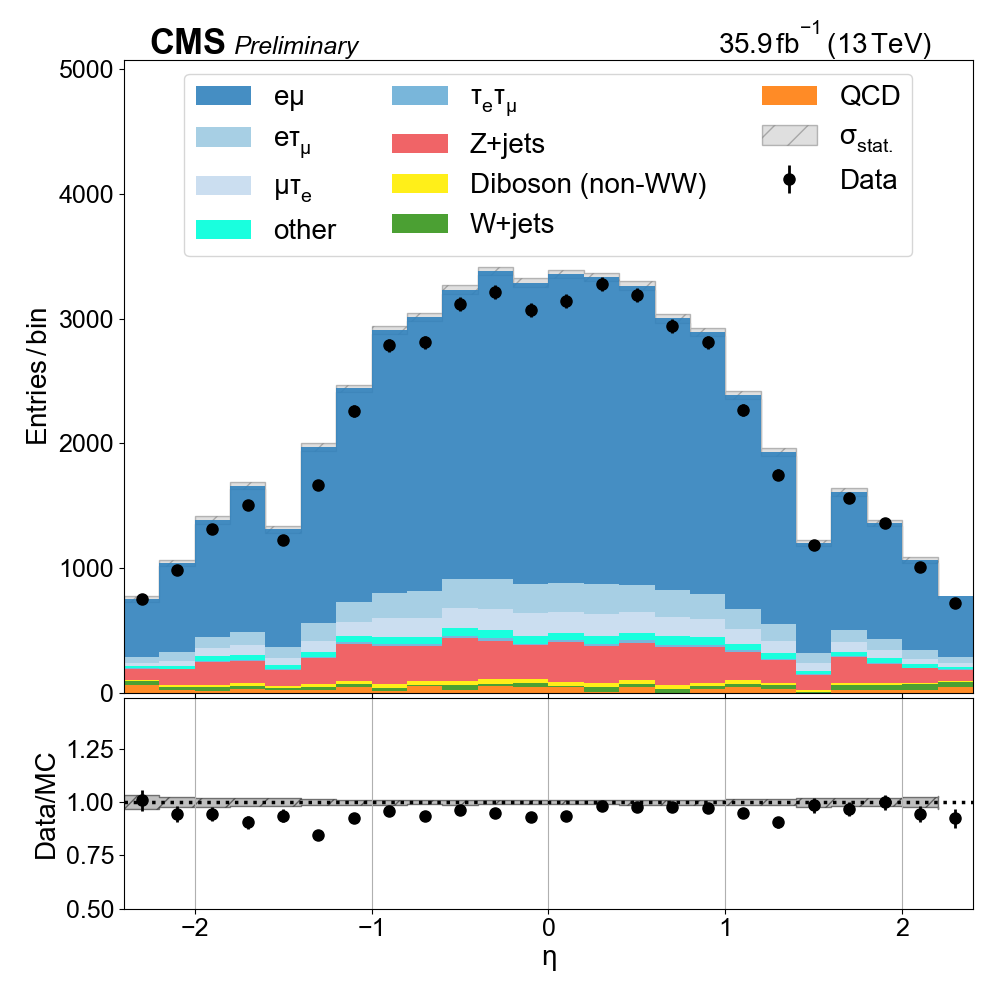
\includegraphics[width=0.4\textwidth]{chapters/Appendix/sectionPlots/figures/data_mc_overlays/emu_2016_cat_gt2_eq0_signal_linear_lepton_lepton2_eta}
    \caption{\pt and $\eta$ distributions for leading (top) and trailing
        (bottom) electrons in the $e\mu$ channel with $N_{j} \geq 2$ and
        $N_{b} = 0$.}
    \label{fig:emu_4_kinematic}
\end{figure}

\begin{figure}[htb!]
    \centering
    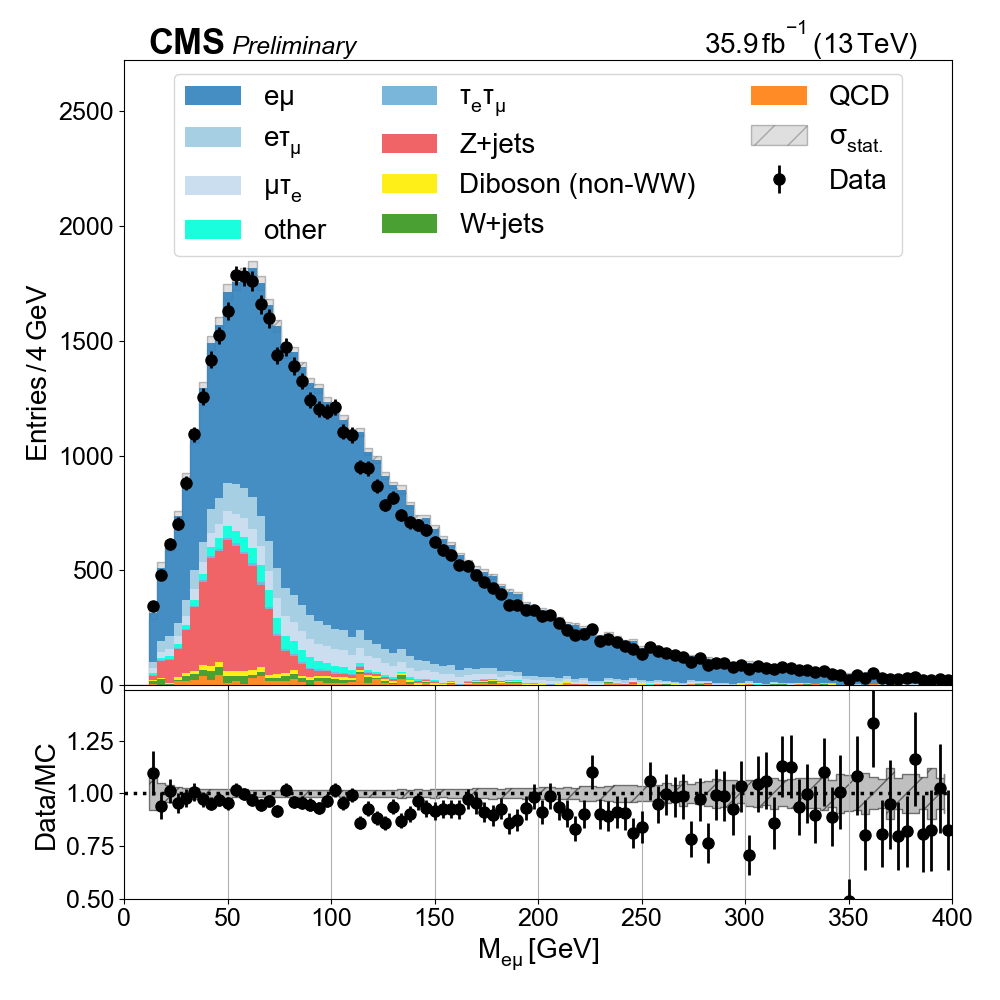
\includegraphics[width=0.3\textwidth]{chapters/Appendix/sectionPlots/figures/data_mc_overlays/emu_2016_cat_gt2_eq0_signal_linear_lepton_dilepton1_mass}
    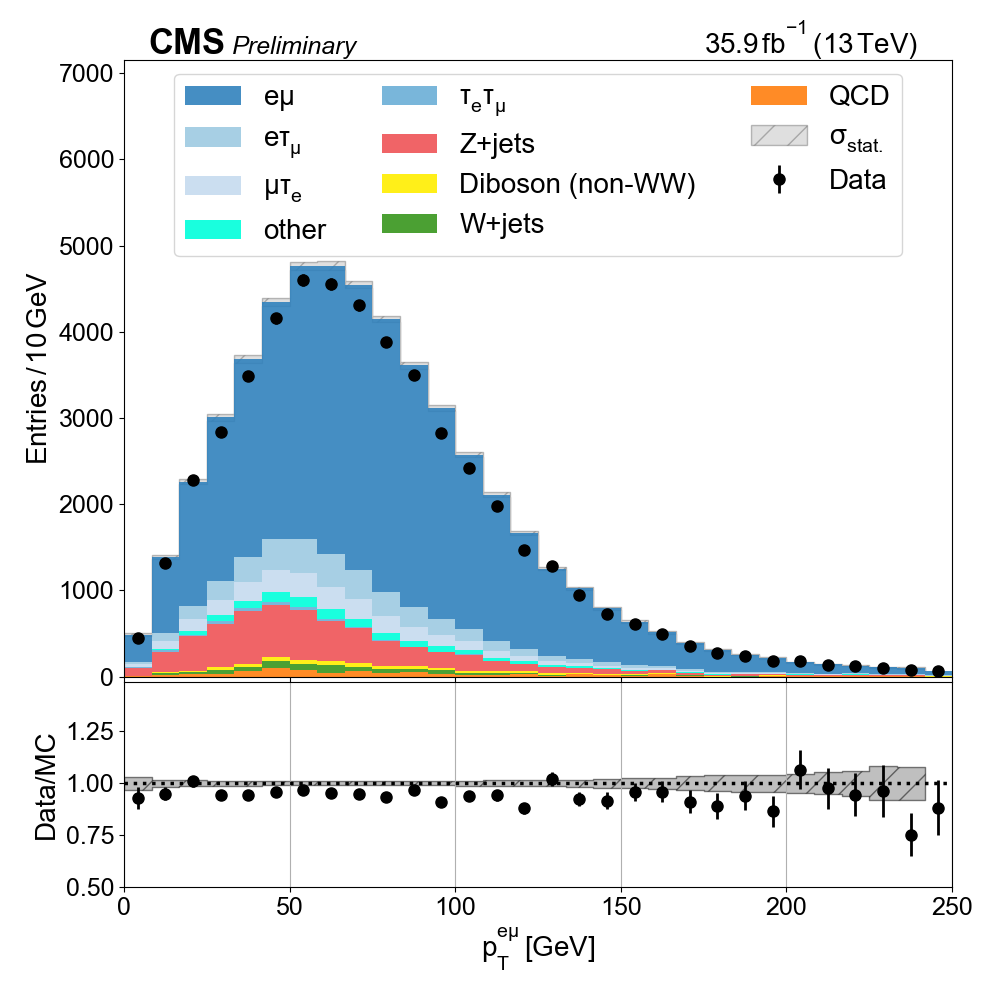
\includegraphics[width=0.3\textwidth]{chapters/Appendix/sectionPlots/figures/data_mc_overlays/emu_2016_cat_gt2_eq0_signal_linear_lepton_dilepton1_pt}
    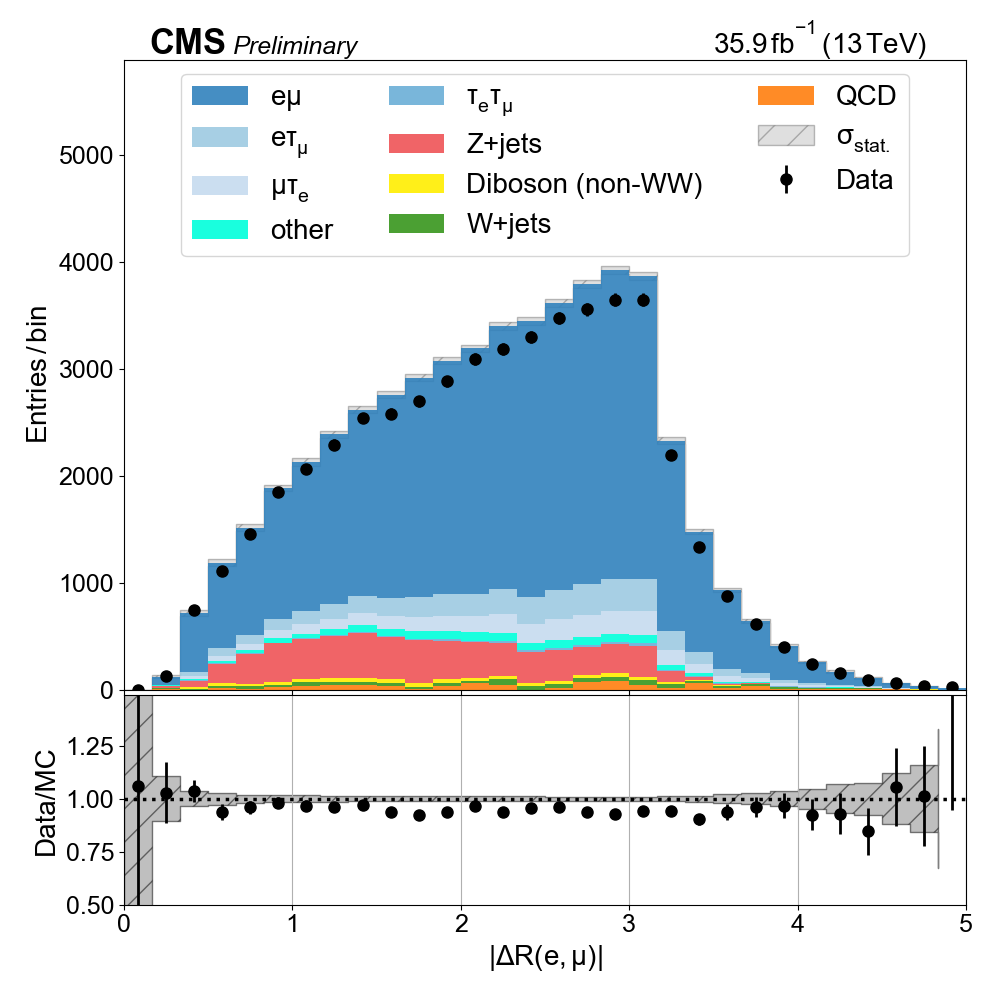
\includegraphics[width=0.3\textwidth]{chapters/Appendix/sectionPlots/figures/data_mc_overlays/emu_2016_cat_gt2_eq0_signal_linear_lepton_dilepton1_delta_r}
    \caption{Dielectron mass, \pt, and $\Delta R$ in the $e\mu$ channel
    with $N_{j} \geq 2$ and $N_{b} = 0$.}
    \label{fig:emu_4_dilepton}
\end{figure}

\begin{figure}[htb!]
    \centering
    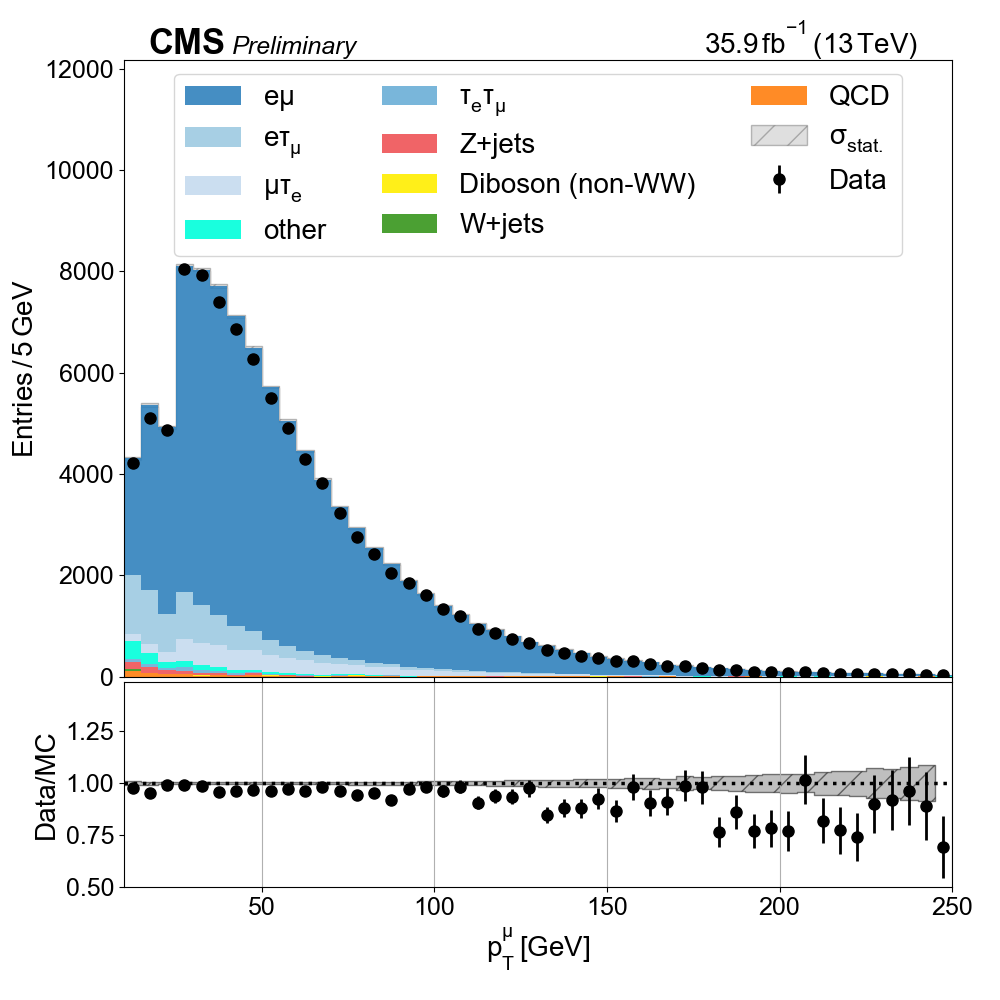
\includegraphics[width=0.4\textwidth]{chapters/Appendix/sectionPlots/figures/data_mc_overlays/emu_2016_cat_gt2_eq1_a_signal_linear_lepton_lepton1_pt}
    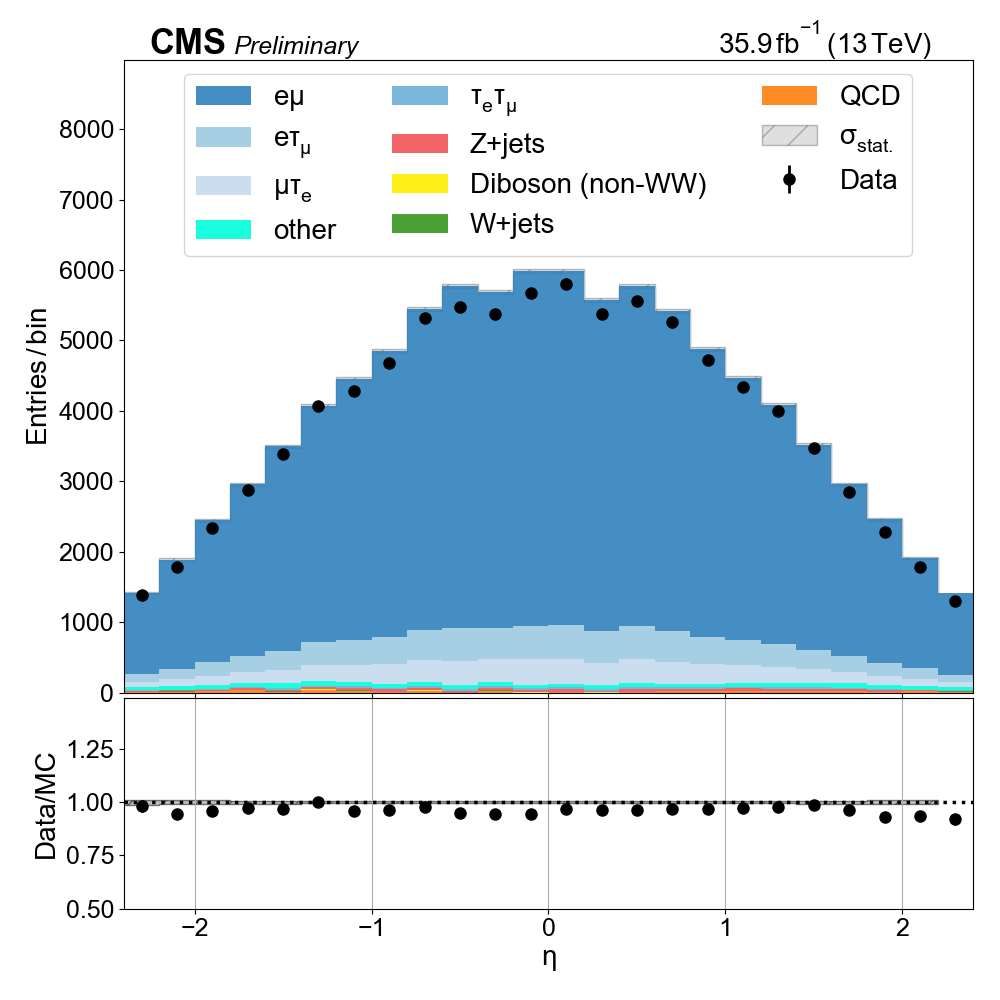
\includegraphics[width=0.4\textwidth]{chapters/Appendix/sectionPlots/figures/data_mc_overlays/emu_2016_cat_gt2_eq1_a_signal_linear_lepton_lepton1_eta}

    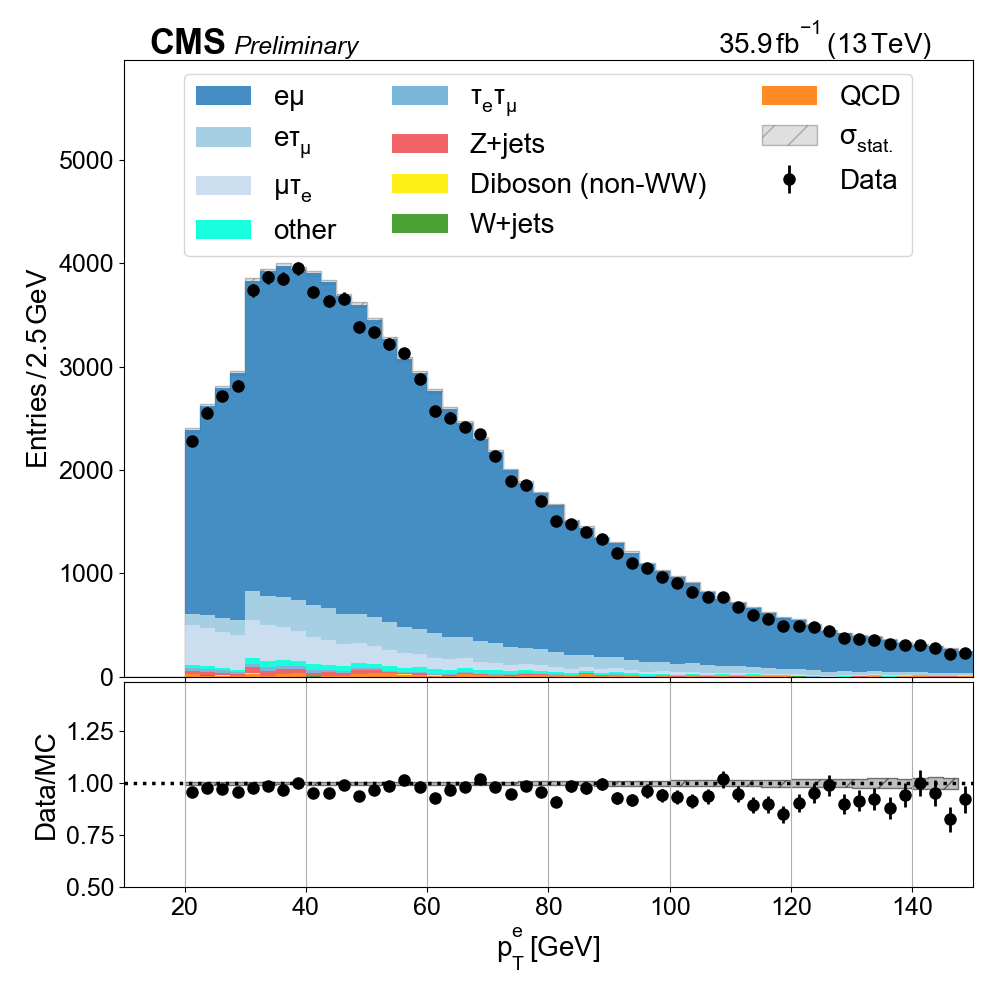
\includegraphics[width=0.4\textwidth]{chapters/Appendix/sectionPlots/figures/data_mc_overlays/emu_2016_cat_gt2_eq1_a_signal_linear_lepton_lepton2_pt}
    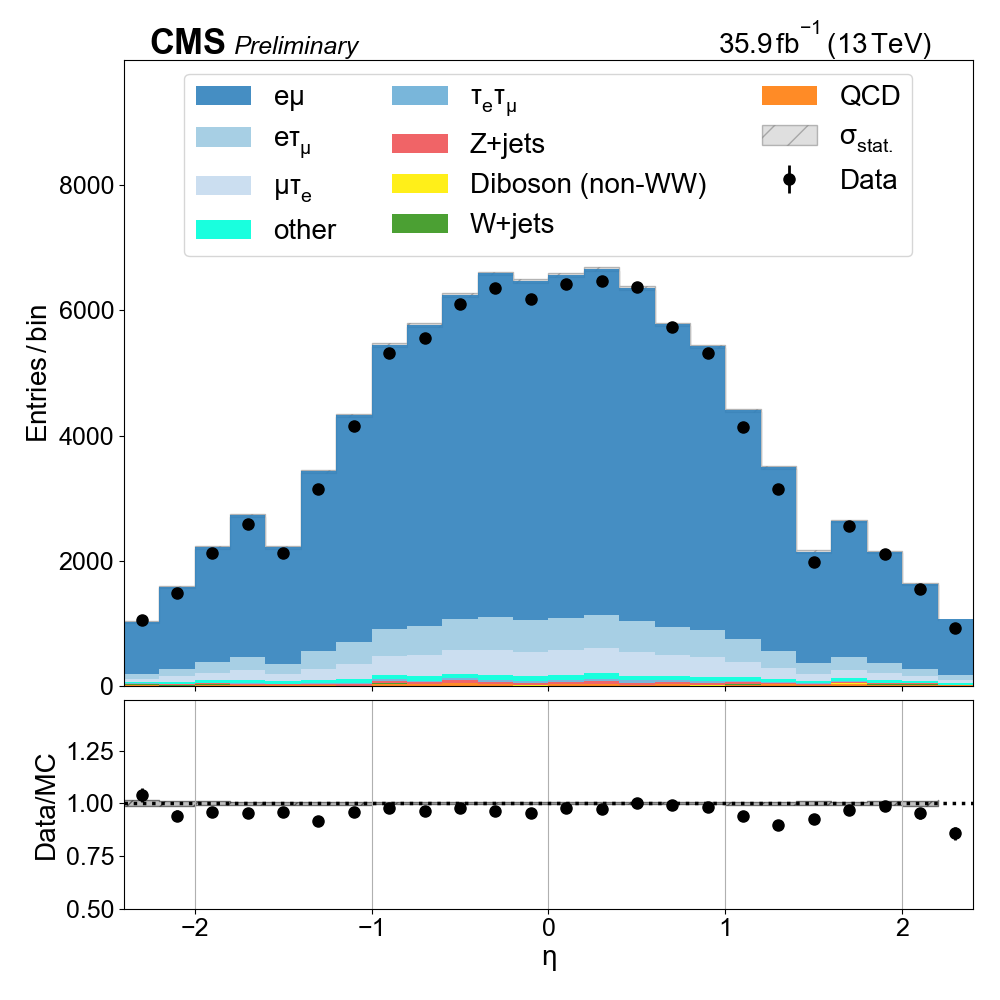
\includegraphics[width=0.4\textwidth]{chapters/Appendix/sectionPlots/figures/data_mc_overlays/emu_2016_cat_gt2_eq1_a_signal_linear_lepton_lepton2_eta}
    \caption{\pt and $\eta$ distributions for leading (top) and trailing
        (bottom) electrons in the $e\mu$ channel with $N_{j} \geq 2$ and
        $N_{b} = 1$.}
    \label{fig:emu_5_kinematic}
\end{figure}

\begin{figure}[htb!]
    \centering
    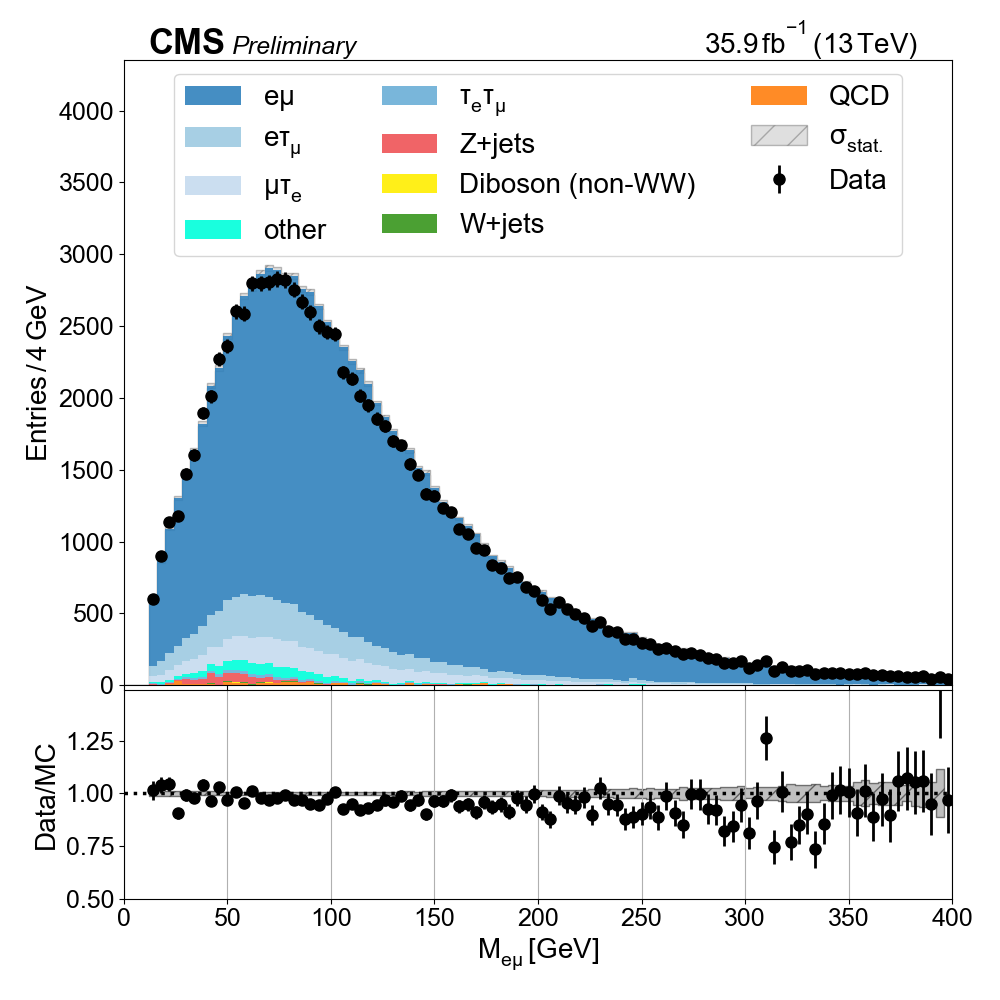
\includegraphics[width=0.3\textwidth]{chapters/Appendix/sectionPlots/figures/data_mc_overlays/emu_2016_cat_gt2_eq1_a_signal_linear_lepton_dilepton1_mass}
    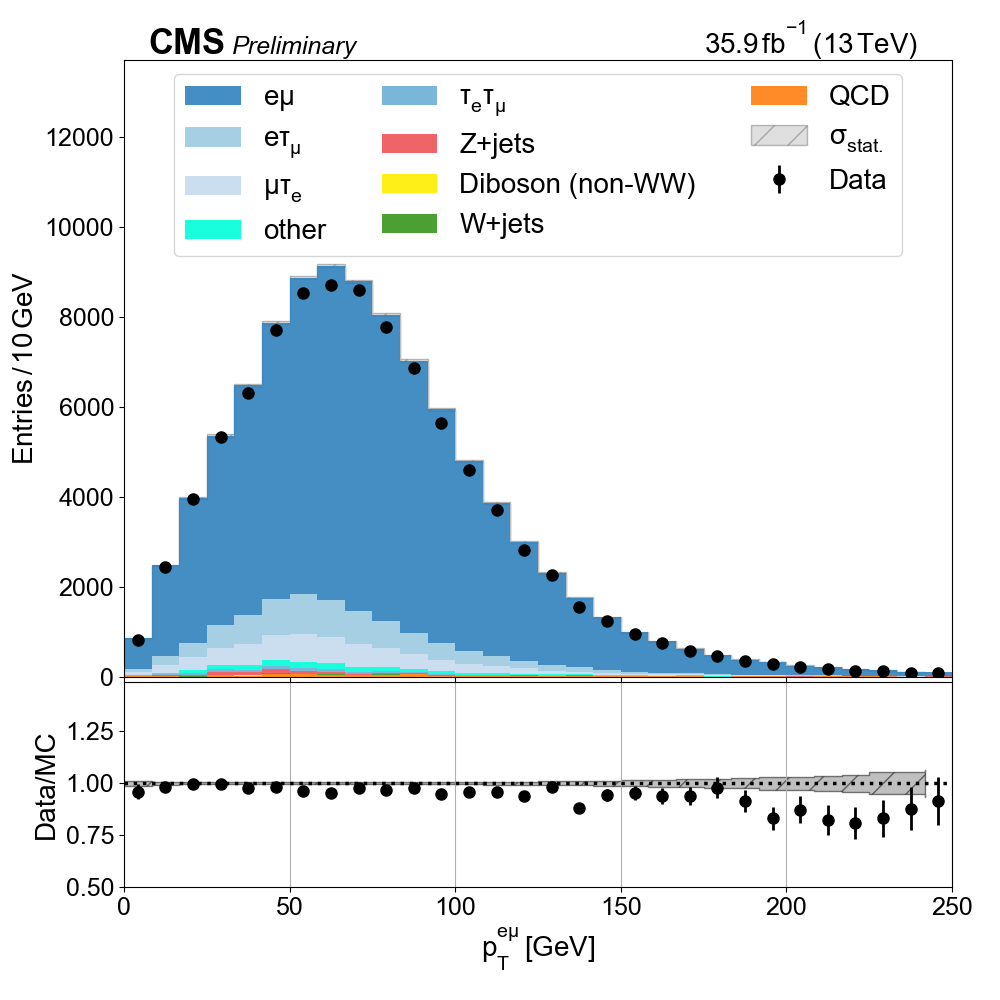
\includegraphics[width=0.3\textwidth]{chapters/Appendix/sectionPlots/figures/data_mc_overlays/emu_2016_cat_gt2_eq1_a_signal_linear_lepton_dilepton1_pt}
    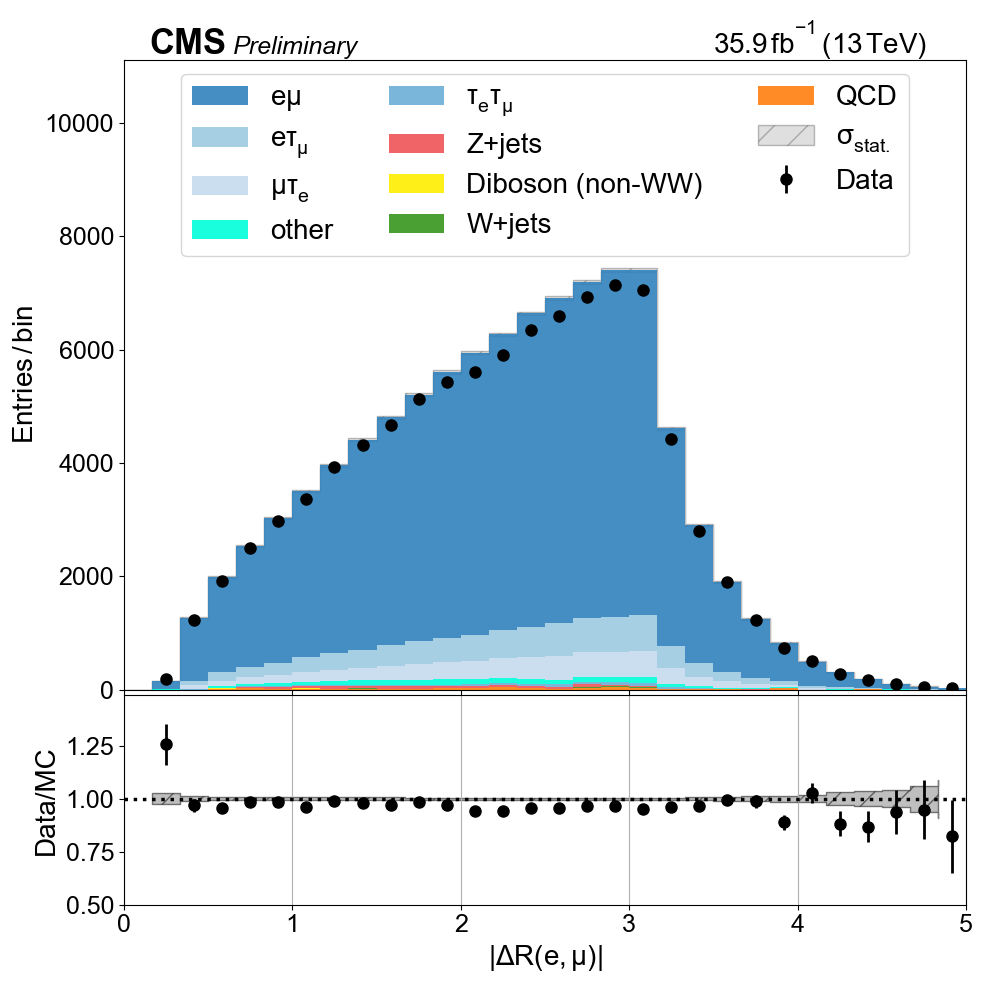
\includegraphics[width=0.3\textwidth]{chapters/Appendix/sectionPlots/figures/data_mc_overlays/emu_2016_cat_gt2_eq1_a_signal_linear_lepton_dilepton1_delta_r}
    \caption{Dielectron mass, \pt, and $\Delta R$ in the $e\mu$ channel
    with $N_{j} \geq 2$ and $N_{b} = 1$.}
    \label{fig:emu_5_dilepton}
\end{figure}

\begin{figure}[htb!]
    \centering
    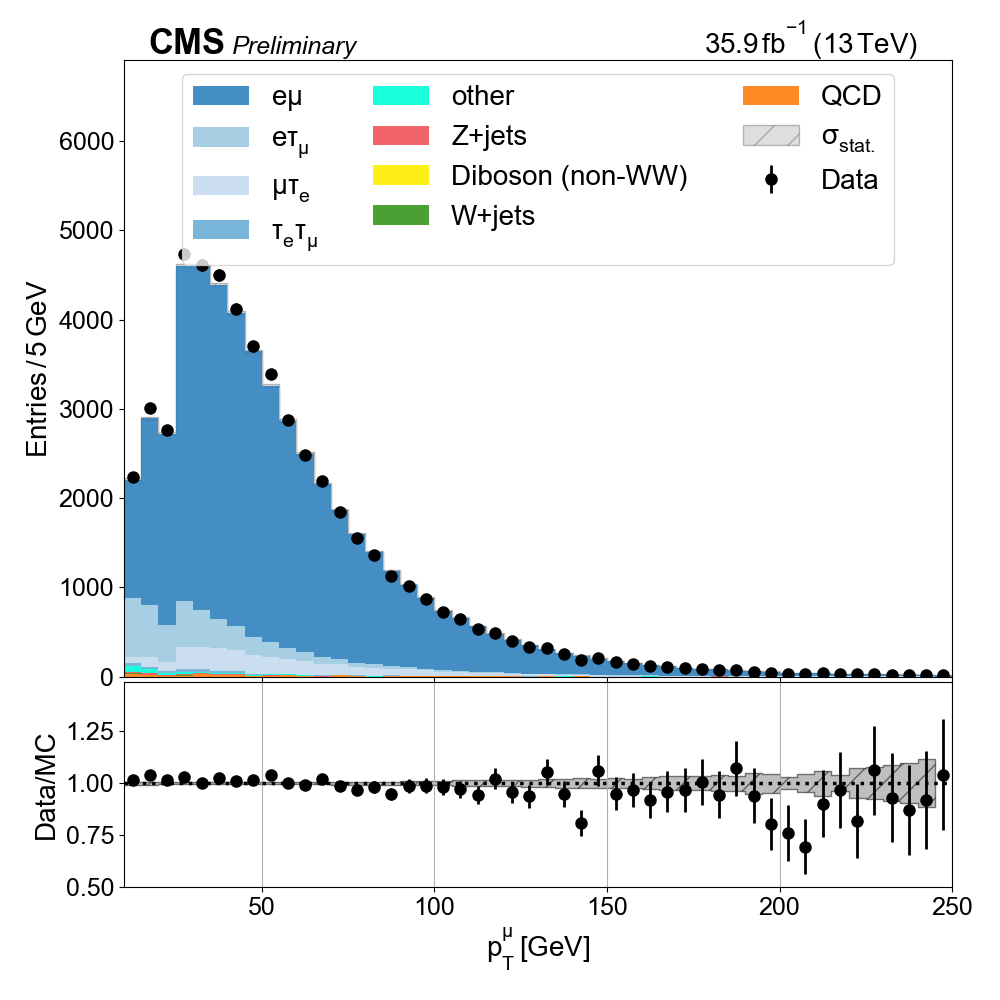
\includegraphics[width=0.4\textwidth]{chapters/Appendix/sectionPlots/figures/data_mc_overlays/emu_2016_cat_gt2_gt2_a_signal_linear_lepton_lepton1_pt}
    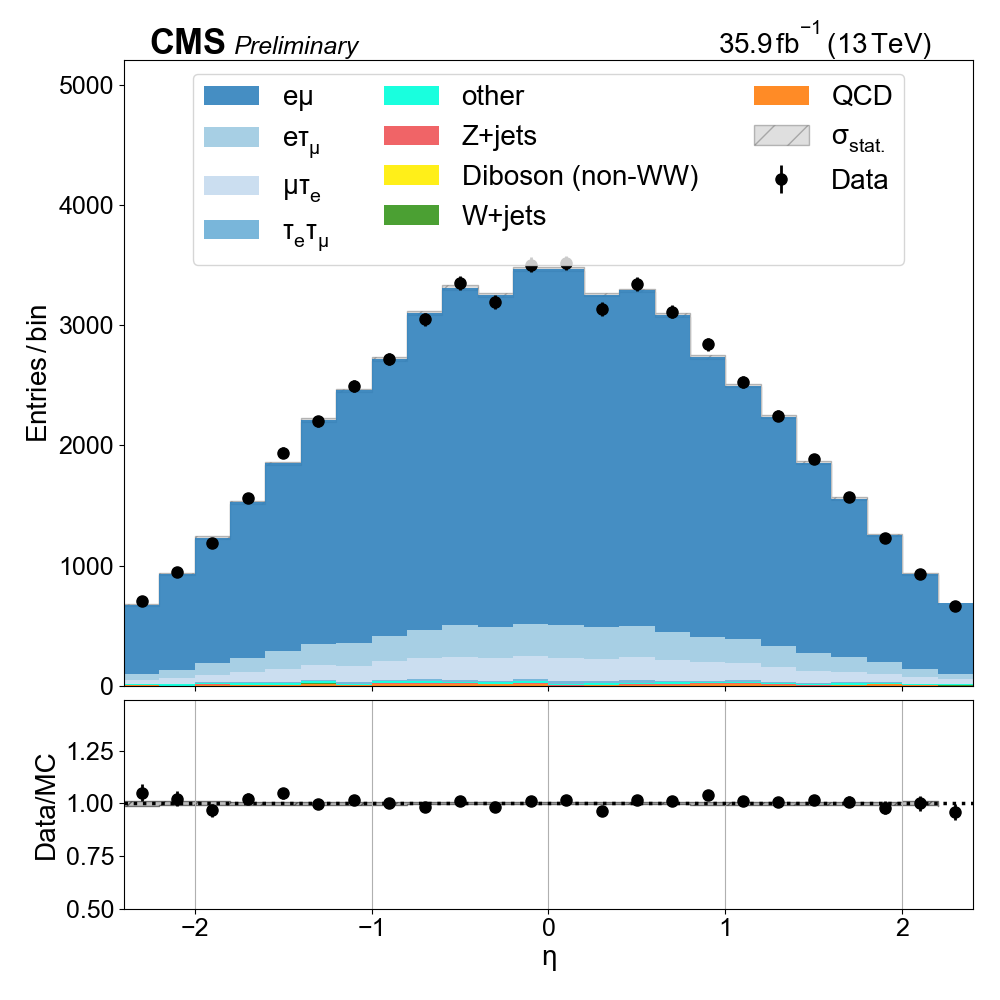
\includegraphics[width=0.4\textwidth]{chapters/Appendix/sectionPlots/figures/data_mc_overlays/emu_2016_cat_gt2_gt2_a_signal_linear_lepton_lepton1_eta}

    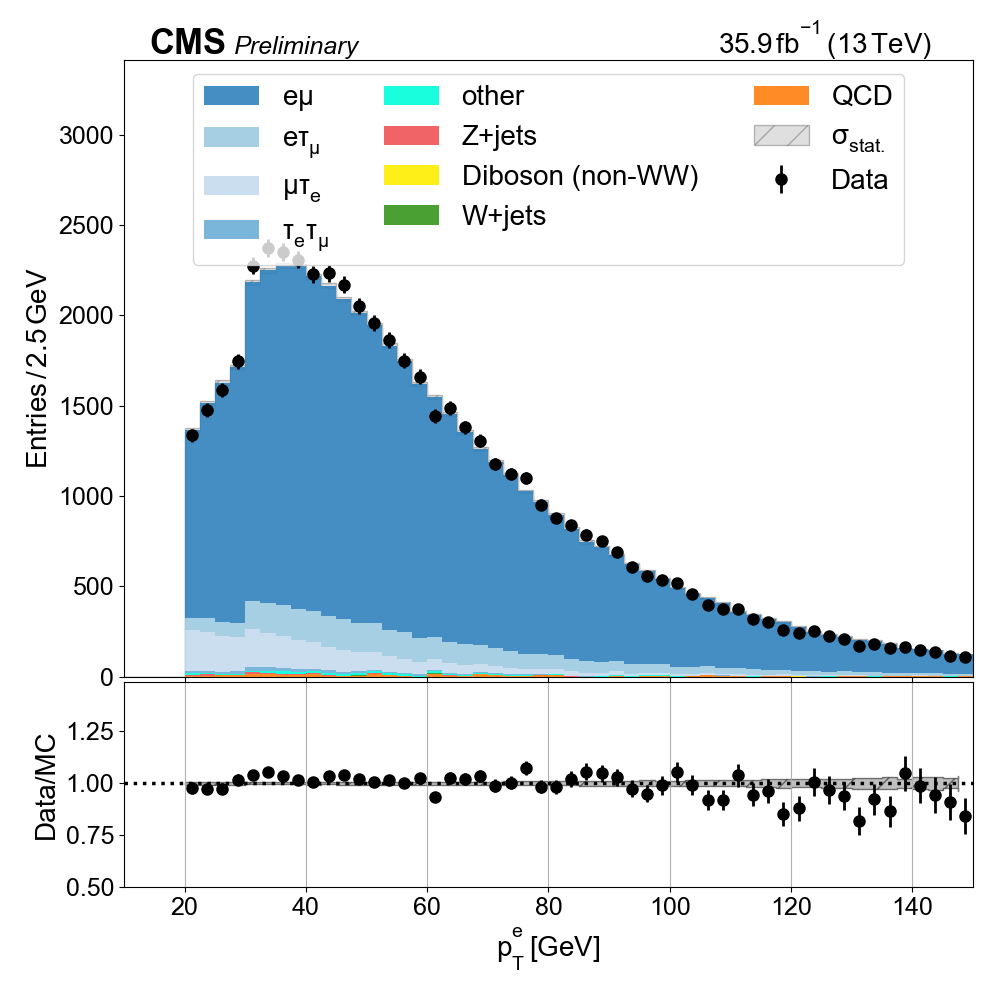
\includegraphics[width=0.4\textwidth]{chapters/Appendix/sectionPlots/figures/data_mc_overlays/emu_2016_cat_gt2_gt2_a_signal_linear_lepton_lepton2_pt}
    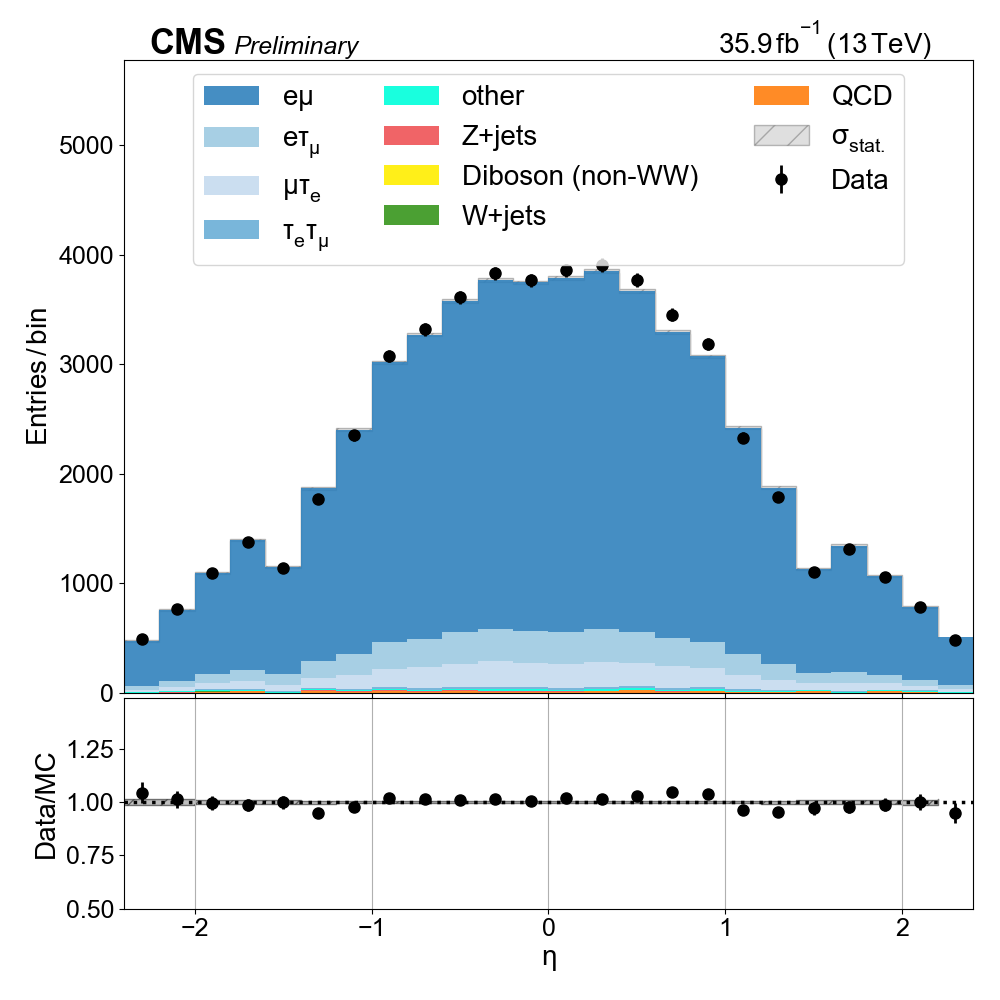
\includegraphics[width=0.4\textwidth]{chapters/Appendix/sectionPlots/figures/data_mc_overlays/emu_2016_cat_gt2_gt2_a_signal_linear_lepton_lepton2_eta}
    \caption{\pt and $\eta$ distributions for leading (top) and trailing
        (bottom) electrons in the $e\mu$ channel with $N_{j} \geq 2$ and
        $N_{b} = 1$.}
    \label{fig:emu_6_kinematic}
\end{figure}

\begin{figure}[htb!]
    \centering
    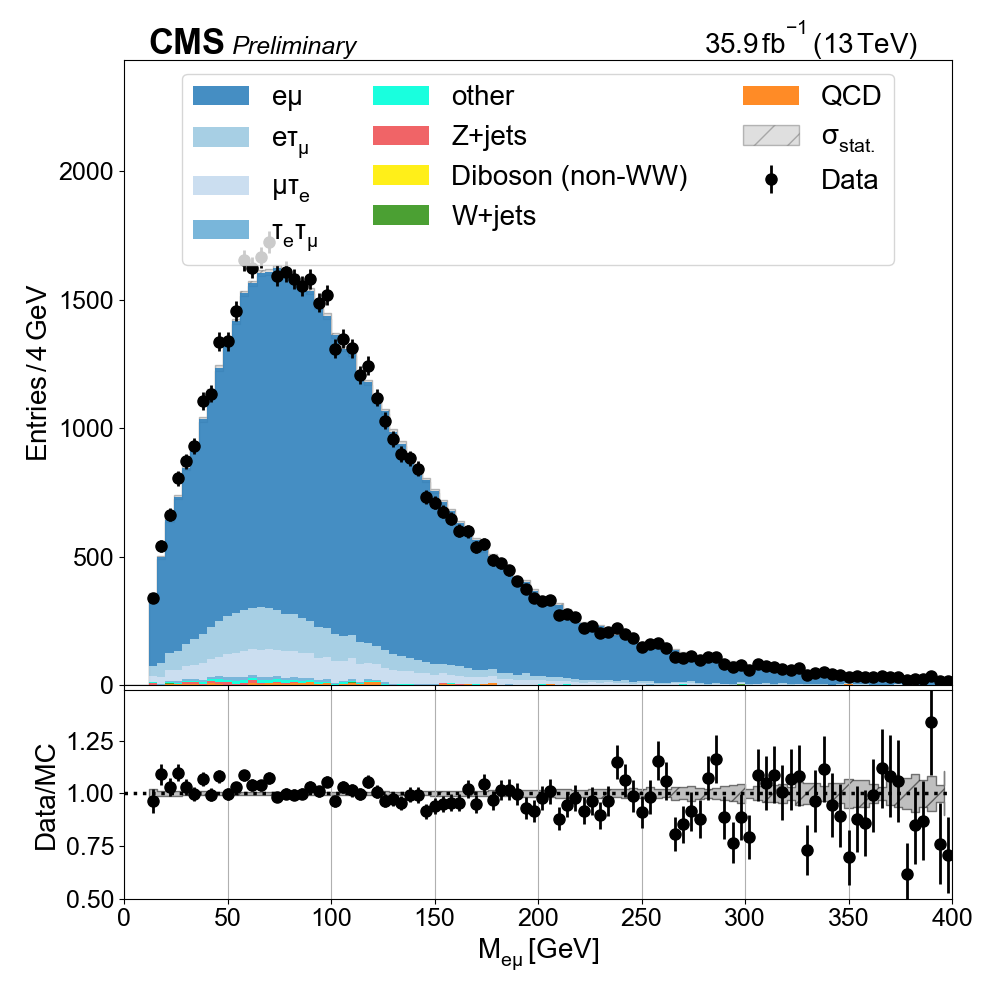
\includegraphics[width=0.3\textwidth]{chapters/Appendix/sectionPlots/figures/data_mc_overlays/emu_2016_cat_gt2_gt2_a_signal_linear_lepton_dilepton1_mass}
    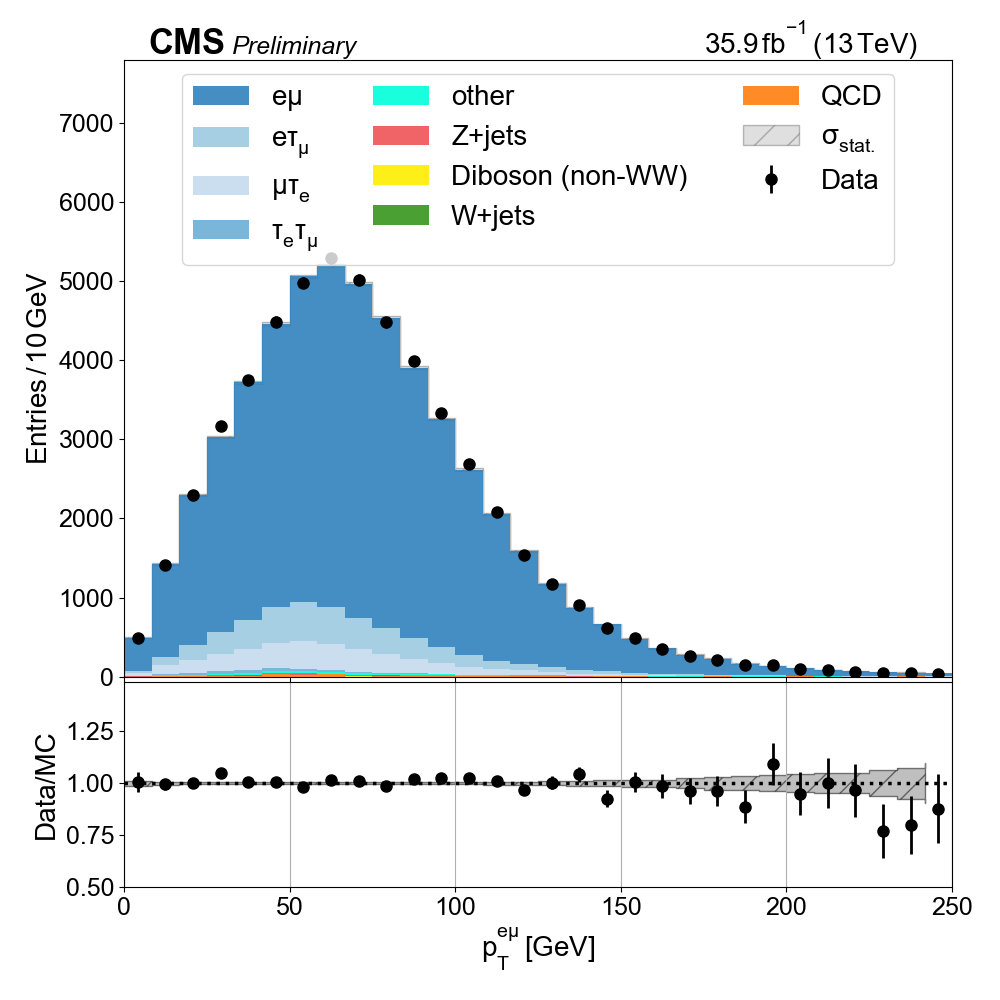
\includegraphics[width=0.3\textwidth]{chapters/Appendix/sectionPlots/figures/data_mc_overlays/emu_2016_cat_gt2_gt2_a_signal_linear_lepton_dilepton1_pt}
    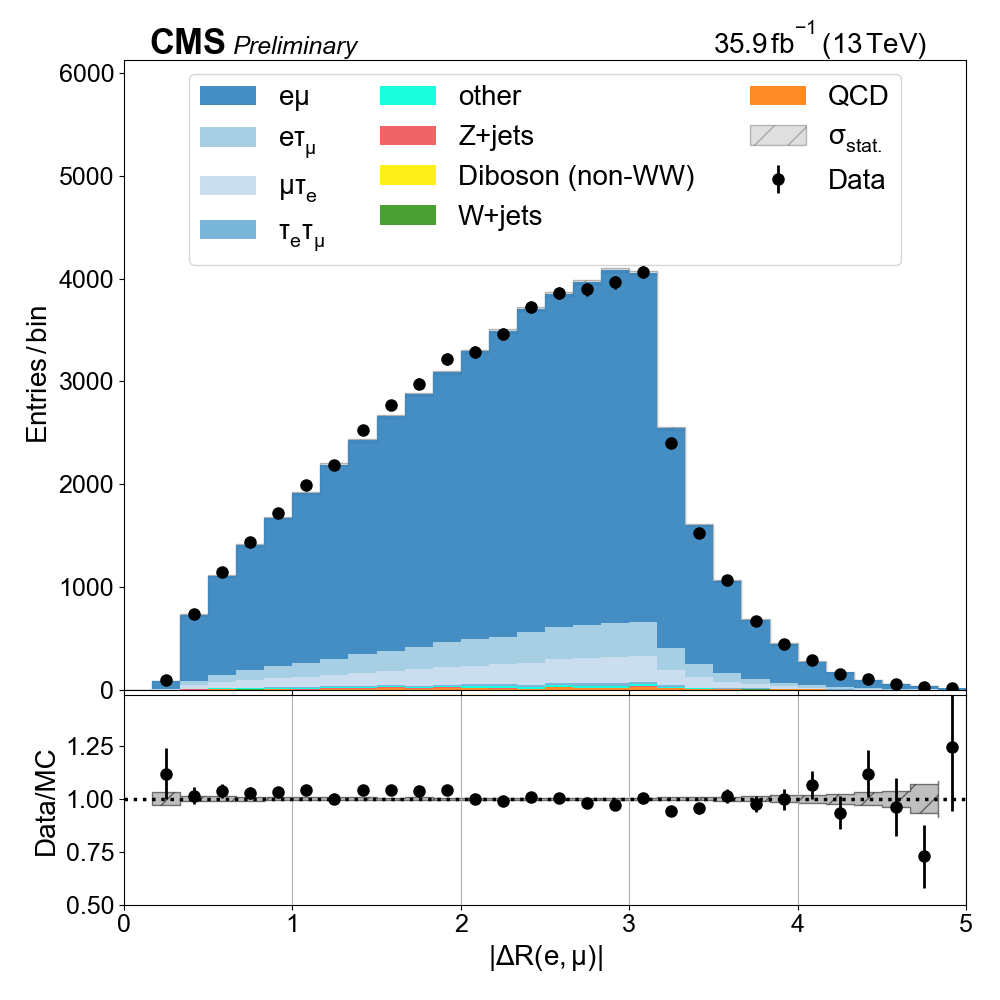
\includegraphics[width=0.3\textwidth]{chapters/Appendix/sectionPlots/figures/data_mc_overlays/emu_2016_cat_gt2_gt2_a_signal_linear_lepton_dilepton1_delta_r}
    \caption{Dielectron mass, \pt, and $\Delta R$ in the $e\mu$ channel
    with $N_{j} \geq 2$ and $N_{b} = 1$.}
    \label{fig:emu_6_dilepton}
\end{figure}

\begin{figure}[htb!]
    \centering
    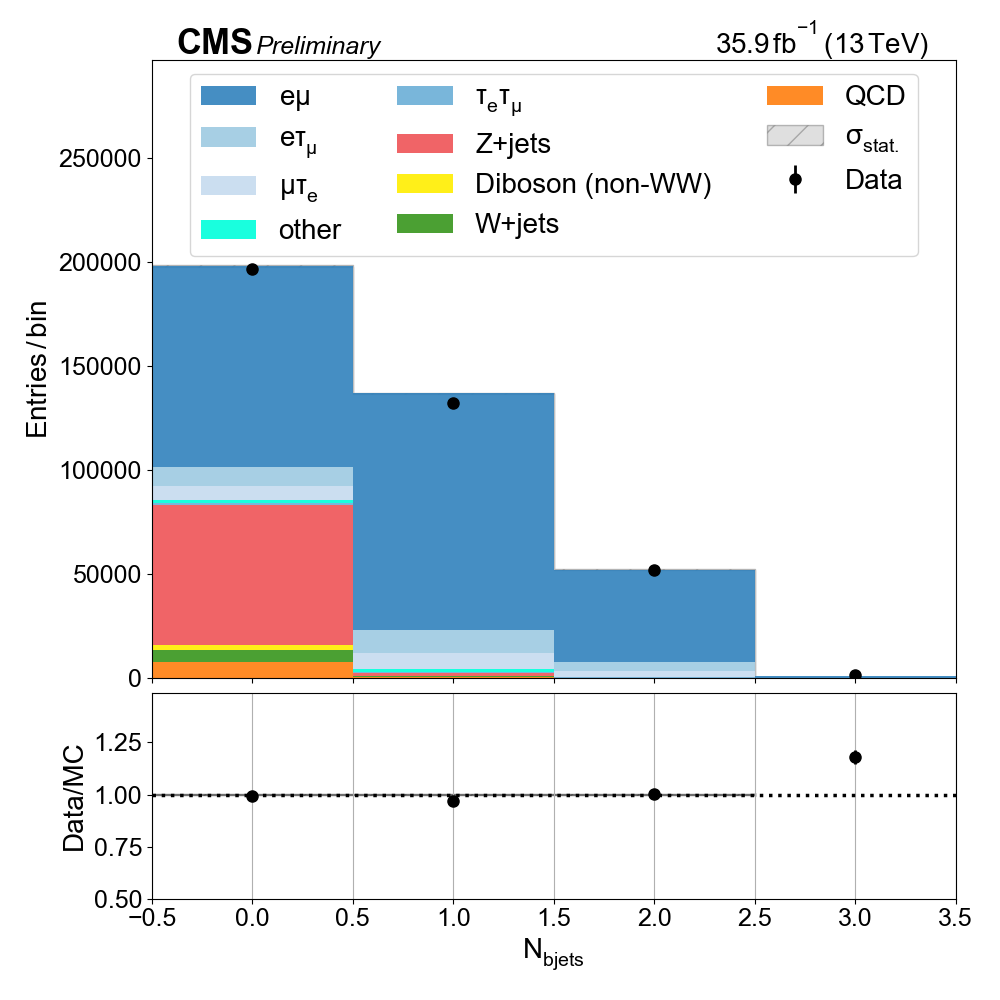
\includegraphics[width=0.4\textwidth]{chapters/Appendix/sectionPlots/figures/data_mc_overlays/emu_2016_inclusive_linear_jet_n_bjets}
    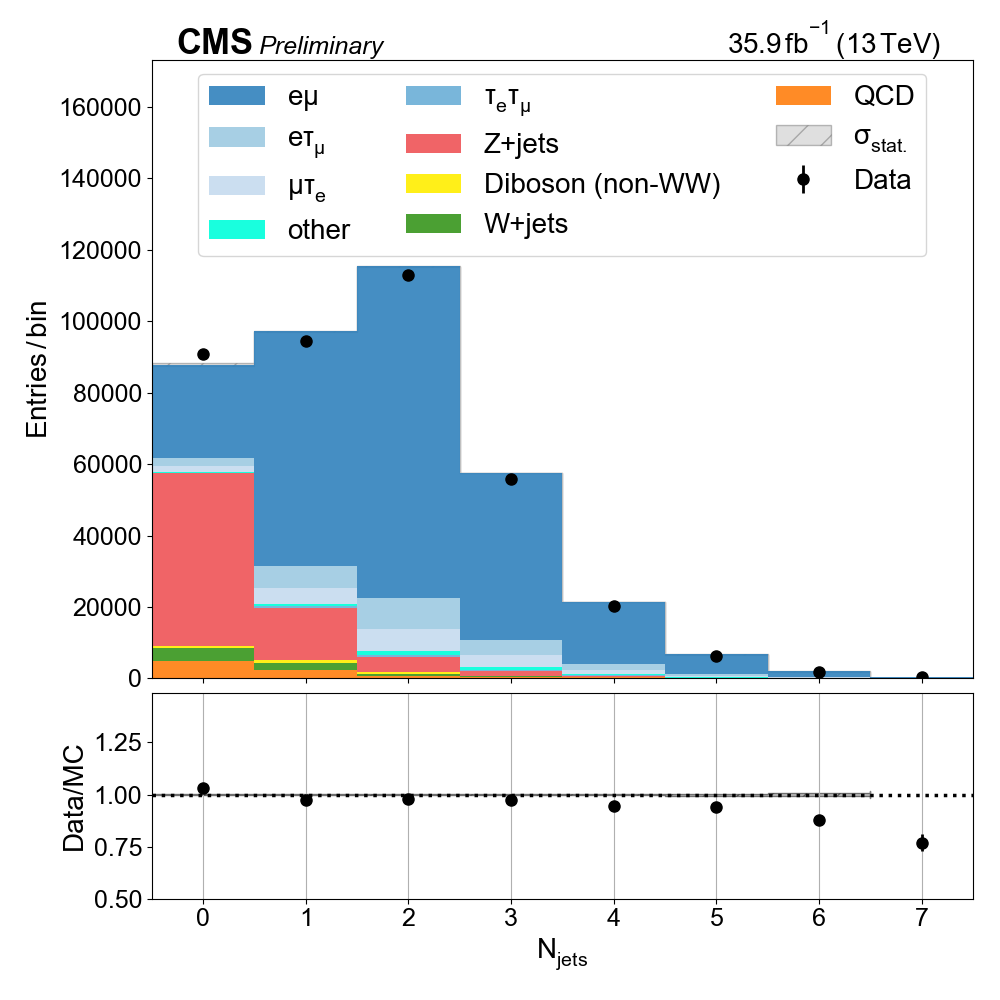
\includegraphics[width=0.4\textwidth]{chapters/Appendix/sectionPlots/figures/data_mc_overlays/emu_2016_inclusive_linear_jet_n_jets}
    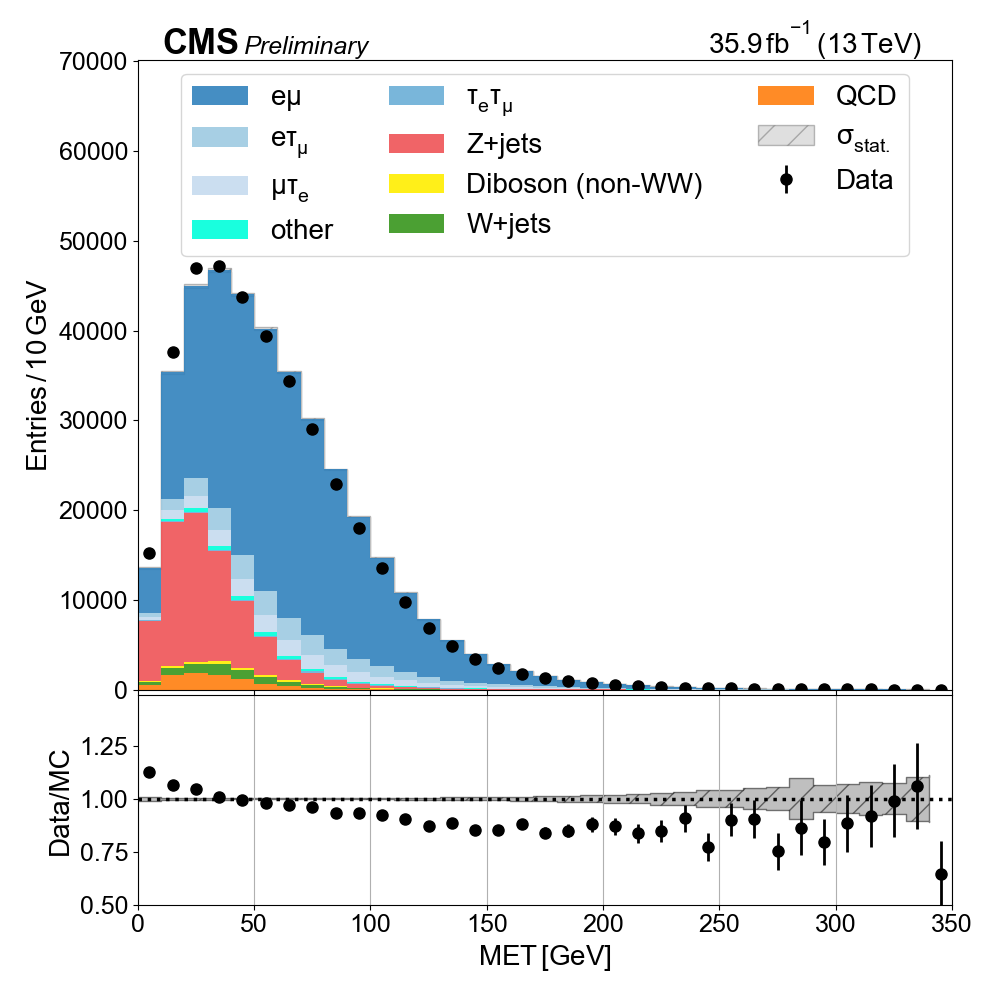
\includegraphics[width=0.3\textwidth]{chapters/Appendix/sectionPlots/figures/data_mc_overlays/emu_2016_inclusive_linear_misc_met_mag}
    \caption{Multiplicity of b tagged jets, non-tagged jets, and MET in
    $e\mu$ channel.}
    \label{fig:emu_jetmet}
\end{figure}

